
\pagestyle{plain} %Estilo da página
\thispagestyle{empty} %Estilo desta página

\newpage
\begin{center}
\textbf{Exercícios de Restrição Orçamentária}\\
\end{center}

\begin{enumerate} %Inicio enumerar
\item Assuma que existam apenas dois bens e suponha que o preço do bem 2 aumentou. Represente graficamente essa mudança. Se sabemos que o consumidor exaure toda a sua renda e prefere consumir mais a menos, esse aumento do preço do bem 2 irá afetar o seu bem-estar de que forma? Isso ocorrerá sempre? \\

\textbf{Resposta:}\\
\begin{center} %Ínicio centralizado
				\begin{tikzpicture}[scale=1]  %Inicio Gráfico e tamanho da escala
						%Eixos
					\draw[->, very thick] (-0.5,0) -- (8.8,0) node[right]{$x_1$}; %Eixo X1
					\draw[->, very thick] (0,-0.5) -- (0,8.8) node[above]{$x_2$}; %Eixo X2					
					    %Retas
					\draw (0,8) -- (6,0) node[below]{$\dfrac{m}{p_{1}}$}; %Primeira Reta
					\draw (6,0) -- (0,5) node[left] {$\dfrac{m}{p_{2}'}$}; %Segunda Reta
						%Complementos gráficos
					\draw[->, very thick, red] (3,4) -- (2,4); %Seta que indica sentido do movimento
					\node[left] at (0,8){$\dfrac{m}{p_{2}}$}; %Dar nome para a intersecção com o eixo X2
				\end{tikzpicture} %Fim do gráfico
				\\
 O gráfico mostra a restrição orçamentária do consumidor quando o preço do bem 2 aumenta.
			\end{center} %Fim centralizado
O aumento do preço do bem 2 só afetará o bem-estar do consumidor caso ele consuma esse bem. Se consumir seu bem-estar diminuirá, se não, permanecerá o mesmo.	
 \\
 	

\item Suponha que os preços de todos os bens aumentem na mesma proporção. Isso é equivalente a uma mudança na renda? Explique.
	\\
	
\textbf{Resposta:}\\

Sim, se todos os preços aumentam na mesma proporção, temos uma nova restrição orçamentária, {$(tp_{1})x_{1}+(tp_{2})x_{2}+...+(tp_{n})x_{n} \leq m$}.
Se, {$t\geq 2$}, o aumento do preços é equivalente a uma diminuição da renda, pois, {$p_{1}x_{1}+p_{2}x_{2}+...+p_{n}x_{n}/2$}. E se, {$t<2$}, o preço cai e a renda aumenta.
\\

\item Suponha que o bem 1 teve o seu preço quadruplicado e o bem 2 teve o seu preço duplicado. O que ocorre com a inclinação da reta orçamentária? Faz sentido dizermos que o bem 1 se tornou relativamente mais barato do que o bem 2?
 \\
 
\textbf{Resposta:}\\

Antes tinhamos uma reta orçamentária com a inclinação {$\frac{-p_{1}}{p_{2}}$} e agora {$\frac{-4p_{1}}{2p_{2}}$}, sendo assim, o preço do bem 1 duplicou em relação ao preço do bem 2, logo o bem 1 ficou mais caro e não mais barato que o bem 2.
\\

\item Suponha que o indivíduo consome apenas dois bens, em que o bem 1 é saúde, medido em termos qualidade (ou seja, quanto mais afastado da origem no eixo horizontal, melhor o serviço de saúde adquirido). O governo resolve prover gratuitamente o nível de saúde {$x_{1} = \overline{s}$} (e apenas esse nível é provido de modo gratuito). Represente a reta orçamentária neste caso
\\

\textbf{Resposta:}\\

\begin{center} %Inicio Centralizado
				\begin{tikzpicture}[scale=1] %Inicio gráfico e tamanho da escala
						%Eixos
					\draw[->, very thick] (-0.1,0) -- (8,0) node[right]{$x_1$}; %Eixo X1
					\draw[->, very thick] (0,-0.1) -- (0,8) node[above]{$x_2$};%Eixo X2
					    %Reta
					\draw (0,5) -- (5,0) node[below]{$\dfrac{m}{p_{1}}$}; 
					
					\node[left] at (0,5){$\dfrac{m}{p_{2}}$}; %Intersecção eixo X2
					\draw[dashed] (2,5) -- (2,0); %Pontilhado eixo X1
                    \draw[dashed] (2,5) -- (0,5); %Pontilhado eixo X2
                    \node[below] at (2,0){$x_{1}=\overline{s}$}; %Intersecção Pontilhado e X1
                    \node[right] at (2,5) {$A$}; %Intersecção pontilhado X1 e X2
					\end{tikzpicture} %Fim do Gráfico
					\\
					
					
\end{center} %Fim centralizado

A Restrição Orçamentária apresentará uma quebra no nivel de saúde {$x_{1}$} = {$\overline{s}$}, pois o consumidor não precisará pagar se consumir nesse nível, podendo gastar sua renda com outros bens. Assim como {$A$} todas as cestas que estiverem no nível {$x_{1}$} = {$\overline{s}$} e {$x_{2}\leq\dfrac{m}{p_{2}}$} são factíveis.
\\

\item Ilustre graficamente a restrição orçamentária para o caso de três bens. O que ocorre com essa restrição se a renda aumentar? E se o preço de um bem aumentar?
\\

\textbf{Resposta:}\\

Para demonstrar a variação de aumento da renda pegamos o bem {$x_2$} e aplicamos na variação da renda, assim, se a renda varia há um aumento no consumo do bem {$x_2$}, mudando de {$m$} para {$m'$}. Já no bem {$x_1$}, ocorre o inverso quando o preço do bem aumenta, há uma diminuição na quantidade consumida, indo de {$b$} para {$b'$}.

\begin{center}

\tdplotsetmaincoords{70}{110}     
\begin{tikzpicture}[scale=1.5,tdplot_main_coords]      
\draw[thick,black,->] (0,0,0) -- (5,0,0) node[anchor=north east]{$x\textit{1}$};       
\draw[thick,black,->] (0,0,0) -- (0,5,0) node[anchor=north west]{$x\textit{2}$};       
\draw[thick,black,->] (0,0,0) -- (0,0,3) node[anchor=south]{$x\textit{3}$};   

		          \draw [thick] (0,0,2) -- (2,0,0);
		          \draw [thick] (0,0,2) -- (1,0,0);
		          \draw [thick] (0,0,2) -- (0,1,0);
		          \draw [thick] (2,0,0) -- (0,1,0);
		          

		          \node [left] at (0,0,2){$\dfrac{m}{\textit{a}}$};
		          \node [below] at (2,0,0) {$\dfrac{m}{\textit{b}}$};
		          \node [below] at (1,0,0) {$\dfrac{m}{\textit{b'}}$};
                   \node [left] at (0.4,0,0.1) {$\nearrow$};
					\node [below] at (0,1,0) {$\dfrac{m'}{\textit{c}}$};
					\node [right] at (0,1.2,0,6) {$\rightarrow$};


     
       
\end{tikzpicture}        
\end{center}
\item Suponha que existam apenas dois bens e o governo resolve controlar os preços desses bens do seguinte modo: o preço é de R\$ 1,00 até 5 unidades adquiridas, e o preço é R\$ 2,00 para unidades adicionais (acima das primeiras 5 unidades adquiridas). Suponha que Carlos tem uma renda de R\$ 10,00.
\\


\paragraph{} a)Ilustre graficamente a reta orçamentária de Carlos.\\

\textbf{Resposta:}\\

\begin{center}
				\begin{tikzpicture}[scale=1] 
						
					\draw[->, very thick] (-0.1,0) -- (8,0) node[right]{$x_1$}; 
					\draw[->, very thick] (0,-0.1) -- (0,8) node[above]{$x_2$};
					\draw (0,6) -- (4,3.5);
					\draw (4,3.5)-- (6.5,0) node[below]{$7,5$};
					\draw[dashed] (4,3.5) -- (4,0);
                    \draw[dashed] (4,3.5) -- (0,3.5);
					\node[left] at (0,6){$7,5$};
                    \node[below] at (4,0){$5$};
                    \node[left] at (0,3.5){$5$};
					\end{tikzpicture}
					\\
\end{center}

\paragraph{} b) Descreva a reta orçamentária em termos algébricos.
\\

\textbf{Resposta:}\\

$m$ = 
$\begin{cases}
x_{1}+2(x_{2}-5)+5=10 \textrm{, se } x_{2}>5, 0\leq x_{1} \leq5\\
2(x_{1}-5)+5+x_{2}=10 \textrm{, se } x_{1}>5, 0\leq x_{2} \leq5
\end{cases}$\\

\item Suponha uma economia com dois bens, denotados por x e y. A reta orçamentária de Maria é {$p^M_xx$} + {$p^M_yy$} = {$m^M$} e a reta orçamentária de João é {$p^J_xx$} + {$p^J_yy$} = {$m^J$}, onde {$p^M_x$} /{$p^J_y$} {$\neq$} {$p^J_x$} /{$p^J_y$}. Ou seja, o custo de mercado entre x e y para Maria é diferente do custo de mercado para João. Maria e João decidem se casar e formar uma família onde a renda dos dois é gasta em conjunto, apesar de que os preços dos bens para cada um deles continuam os mesmos de antes.

\paragraph{} a) Defina a restrição orçamentária do casal.
\\

\textbf{Resposta:}\\

A restrição orçamentária do casal é: {$p_{x}x$} + {$p_{y}y$} = $m$.\\

Onde:\\
$p_{x}$ = min{$\lbrace$}{$p^M_x$},{$p^J_x$}{$\rbrace$},\\
$p_{y}$ = min{$\lbrace$}{$p^M_y$},{$p^J_y$}{$\rbrace$},\\
{$m$} = {$m^M$} e {$m^J$}.\\

\paragraph{} b) Haverá especialização na compra dos bens?\\

\textbf{Resposta:}\\

Sim, pois se Maria tem acesso ao preço do bem x mais barato e João ao preço do bem y, logo Maria se especializará na compra do bem x e joão na compra do bem y.\\

\newpage

\begin{center}
\textbf{Exercícios de Preferência}\\
\end{center}

\item[1.] Suponha um consumidor que tenha preferências definidas entre cestas compostas por dois bens do seguinte modo: se {$(x_{1},x_{2})$}{$\geq$}{$(y_{1},y_{2})$} (ou seja, {$x_{1}$}{$\geq$}{$y_{1}$} e {$x_{2}$}{$\geq$}{$y_{2})$}, então x {$\succeq$} y.\\

\paragraph{}a) Mostre como são as relações de preferência estrita e de indiferença associadas a {$\succeq$}.\\

\textbf{Resposta:}\\
 
Relação de Preferência Estrita {$"\succ"$} é definida pela relação binária {$"\succeq"$}. Significa que vale {$(x_{1},x_{2})$}{$\succeq$}{$(y_{1},y_{2})$} e que não vale {$(y_{1},y_{2})$}{$\succeq$}{$(x_{1},x_{2})$}.  Assim, ou {$(y_{1}<x_{1})$} ou {$(y_{2}<x_{2})$}. Então, {$(x_{1},x_{2})$}{$\succ$}{$(y_{1},y_{2})$} significa que {$(x_{1}$}{$\geq$}{$y_{1})$} e {$(x_{2}$}{$\geq$}{$y_{2})$}, com pelo menos uma das cestas valendo de modo estrito.\\

Relação de Indiferença {$"\sim"$} é definida pela relação binária {$"\succeq"$}. Significa que vale {$(x_{1},x_{2})$}{$\succeq$}{$(y_{1},y_{2})$} assim como {$(y_{1},y_{2})$}{$\succeq$}{$(x_{1},x_{2})$}. No primeiro caso, temos que {$(x_1\geq y_1)$} e {$(x_2\geq y_2)$} e no segundo caso temos que {$(x_1\leq y_1)$} e {$(x_2\leq y_2)$}. Portanto, {$(x_1,x_2)$}{$\sim$}{$(y_1,y_2)$} significa que {$x_1 = y_1$} e {$x_2 = y_2$}, para a preferência definida neste exercécio (observe então que a única cesta indiferente à cesta (x1,x2) é ela própria. 



\paragraph{} b) Essas preferências são(justifique sua resposta):\\

\paragraph{} i) Completas?\\ 
\paragraph{} ii) Transitivas?\\
\paragraph{} iii) monótonas?\\
\paragraph{} iv)Convexas\\

\item[2.] O técnico de vôlei Bernardo acha que os jogadores devem ter três qualidades: altura, agilidade e obediência. Se o jogador A é melhor que o jogador B em duas dessas três características, então Bernardo prefere A a B. Para os outros casos, ele é indiferente entre A e B. Carlos mede {$2,08m$}, é pouco ágil e obediente. Luis mede {$1,90m$}, é muito ágil, e muito desobediente. Paulo mede {$1,85m$}, é ágil, e extremamente obediente.\\


\paragraph{}a) Bernardo prefere Carlos ou Luis? Bernardo prefere Luis ou Paulo? Bernardo prefere Carlos ou Paulo?\\

\textbf{Resposta:}\\

Carlos - Altura: 2,08m; Agilidade: pouco agil; Obediência: obediente.\\

Luis - Altura: 1,90m; Agilidade: muito ágil; Obediência: muito desobediente.\\

Paulo - Altura: 1,85m; agilidade: normal; Obediência: extremamente obediente\\

Carlos {$\succ$} Luis; Luis {$\succ$} Paulo e Paulo {$\succ$} Carlos\\

\paragraph{}b) As preferências do técnico são transitivas?\\

\textbf{Resposta:}\\

Não, não são transitivas. Pois Carlos não é preferível a Paulo.\\

\paragraph{}c) Depois de perder vários campeonatos, Bernardo decide mudar sua forma de comparar os jogadores. Agora ele prefere o jogador A ao jogador B se A é melhor do que B nas três características. Ele é indiferente entre A e B se eles têm todas as três caracterésticas iguais. Para todas as outras possibilidades, Bernardo diz que não é possível comparar os jogadores. As novas preferências de Bernardo são: completas? transitivas? reflexivas? Justifique.

\textbf{Resposta:}\\

Não são completas, pois o treinador não consegue mais decidir entre Carlos e Luis, já que Carlos é mais alto e mais obediente, porém menos agil que Luis.\\
São transitivas pois agora o treinador consegue comparar os jogadores, então A{$\succeq$}B e B{$\succeq$}C e A{$\succeq$}C.\\
São reflexivas, pois o treinador é indiferente ao mesmo jogador, logo A{$\succeq$}A\\

\item[3.] Mostre que a preferência lexicográfica é completa, reflexiva e transitiva.\\

\textbf{Resposta:}\\

Sejam as cestas X = {$(x_1,x_2)$} e Y = {$(y_1,y_2)$} bens quaisquer.\\ 

Completa: Se {$x_1 > y_1$}, então, {$x \succ y$}, ou seja, {$x \succeq y$}. Se {$y_1 > x_1$}, então, {$y \succ x$}, ou seja, {$y \succeq x$}. No caso em {$x_1 = y_1$}, olhamos o segundo bem: se {$x_2 > y_2$}, então {$x \succ  y$}, ou seja, {$x \succeq y$}. Se {$y_2 > x_2$}, então {$y \succ x$}, ou
seja, {$y \succeq x$}. Por fim, se {$x_1 = y_1$} e {$x_2 = y_2$}, então {$x \sim y$}, ou seja, {$x \succeq y$}. Dessa forma, em termos da preferência lexicográfica, é sempre possível comparar as cestas X e Y , o que significa que ela é completa.\\

Reflexiva: Para uma cesta X = {$(x_1, x_2)$} qualquer, temos sempre que {$x_1 = x_1$} e {$x_2 = x_2$}, ou
seja, {$x\sim x$}, logo {$x \succeq x$}, o que mostra que a preferência lexicográfica é reflexiva.\\

Transitiva: Considere as cestas X = {$(x_1, x_2)$}, Y = {$(y_1, y_2)$} e Z = {$(z_1, z_2)$}, sendo {$x \succeq y$} e {$y \succeq z$}.
\begin{enumerate}

\item {$x \sim y$} implica que x = y. {$y \sim z$} implica que y = z. Logo, {$x \sim z$} quer dizer que x = z. Ou seja, {$ x\succeq z$}.

\item {$x \succ y$} implica que {$ x_{1} > y_{1}$} ou que {$x_{1} = y_{1}$} e {$x_{2} > y_{2}$}. {$y \sim z$} implica que {$y = z$}. Logo, ou {$x_{1} > z_{1}$} ou {$x_{1} = z_{1}$} e {$x_{2} > z_{2}$}. Mais especificamente {$x \succ z$}. Assim, {$ x\succeq z$}.

\item {$x \sim y$} implica que x = y.  {$y \succ z$} implica que {$ y_{1} > z_{1}$} ou que {$y_{1} = z_{1}$} e {$y_{2} > z_{2}$}. Logo {$x \succ z$} pois {$ x_{1} > z_{1}$} ou que {$x_{1} = z_{1}$} e {$x_{2} > z_{2}$}. Então, {$ x\succeq z$}.

\item {$x \succ y$} implica que  {$ x_{1} > y_{1}$} ou que {$x_{1} = y_{1}$} e {$x_{2} > y_{2}$}. {$y \succ z$} {$ y_{1} > z_{1}$} ou que {$y_{1} = z_{1}$} e {$y_{2} > z_{2}$}. logo {$x \succ z$} pois {$ x_{1} > z_{1}$} ou que {$x_{1} = z_{1}$} e {$x_{2} > z_{2}$}. logo,{$ x\succeq z$}. \\
 
\end{enumerate}


\item[4.] Considere a utilidade u{$(x_1,x_2)$} = {$x^{0,5}_1$} {$x^{0,5}_2$}.\\

\paragraph{}a) Calcule as utilidades marginais dos bens 1 e 2. Verifique que são decrescentes. Qual seria a interpretação de utilidades marginais decrescentes?\\

\textbf{Resposta:}\\

\paragraph{}b) Calcule as utilidades marginais dos bens 1 e 2 para a funcão de utilidade {$\overline{u}$}{$(x_1,x_2)$} = {$x^2_1x^2_2$}. Verifique que são crescentes.\\

\textbf{Resposta:}\\

\paragraph{}c) Mostre que u e {$\overline{u}$} representam a mesma preferência. O que isso implica a respeito de a utilidade marginal ser decrescente ou crescente?\\

\textbf{Resposta:}\\

\item[5.] Desenhe as curvas de indiferença para as seguintes utilidades:\\


\paragraph{}a) Utilidade Linear: u{$(x_1,x_2)$} = {$ax_1 + bx_2$}, a,b {$>$} 0.\\


\textbf{Resposta:}\\

\begin{center} %Centralização do gráfico a ser desenhado
				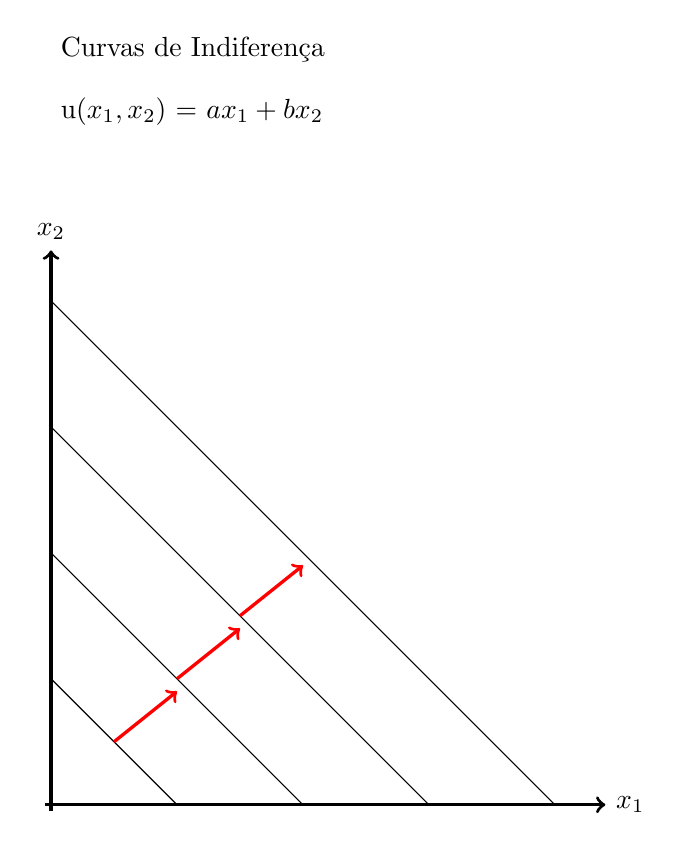
\begin{tikzpicture}[scale=0.8] %Início do desenho e definição da escala
						%Eixos
					\draw[->, very thick] (-0.1,0) -- (8.8,0) node[right]{$x_1$}; %Eixo X1
					\draw[->, very thick] (0,-0.1) -- (0,8.8) node[above]{$x_2$}; %Eixo X2
						%Retas
					\draw (0,8) -- (8,0);
					\draw (0,6) -- (6,0);
					\draw (0,4) -- (4,0);
					\draw (0,2) -- (2,0);
					\draw (0,12) node [right] {Curvas de Indiferença};
					\draw (0,11) node [right] {u{$(x_1,x_2)$} = {$ax_1 + bx_2$}};
					\draw[->, very thick, red] (1,1) -- (2,1.8); 
					\draw[->, very thick, red] (2,2) -- (3,2.8);
			        \draw[->, very thick, red] (3,3) -- (4,3.8);
					
				\end{tikzpicture}\\
				 
			\end{center} 


\paragraph{} b)  Utilidade de Leontief: u{$(x_1,x_2)$} = {$min \{ax_1,bx_2\}$}, a, b {$>$} 0.\\

\textbf{Resposta:}\\

\begin{center} %Centralização do gráfico a ser desenhado
				\begin{tikzpicture}[scale=0.8] %Início do desenho e definição da escala
						%Eixos
					\draw[->, very thick] (-0.1,0) -- (8.8,0) node[right]{$x_1$}; %Eixo X1
					\draw[->, very thick] (0,-0.1) -- (0,8.8) node[above]{$x_2$}; %Eixo X2
						%Retas
					
					\draw (1.5,2) -- (7,2);
					\draw (1.5,2) -- (1.5,7);
					
					\draw (2.5,3) -- (7,3);
					\draw (2.5,3) -- (2.5,7);
				
				    \draw (3.5,4) -- (7,4);
					\draw (3.5,4) -- (3.5,7);
					
					
					\draw[->, very thick, red] (3,2.5) -- (3.5,2.9); 
					\draw[->, very thick, red] (1.7,5.2) -- (2.2,5.5); 
					
					\draw[->, very thick, red] (4,3.5) -- (4.5,3.9); 
					\draw[->, very thick, red] (2.7,5.2) -- (3.2,5.5);
					
					\draw (0,12) node [right] {Curvas de Indiferença};
					\draw (0,11) node [right] {u{$(x_1,x_2)$} = min{$\{ax_1, bx_2\}$}};
				\end{tikzpicture}\\
				
				 
			\end{center} 
			
			
\paragraph{} c) Utilidades com um Bem Neutro: u{$(x_1, x_2)$} = {$x_1$} e u{$(x_1, x_2)$} = {$x_2$}.

\textbf{Resposta:}\\

\begin{center} %Centralização do gráfico a ser desenhado
				\begin{tikzpicture}[scale=0.8] %Início do desenho e definição da escala
						%Eixos
					\draw[->, very thick] (-0.1,0) -- (8.8,0) node[right]{$x_1$}; %Eixo X1
					\draw[->, very thick] (0,-0.1) -- (0,8.8) node[above]{$x_2$}; %Eixo X2
						%Retas
					\draw (1.7,0) -- (1.7,4);
					\draw (2.8,0) -- (2.8,4);
					\draw (3.9,0) -- (3.9,4);
					\draw (0,12) node [right] {Curvas de Indiferença};
					\draw (0,11) node [right] {u{$(x_1, x_2)$} = {$x_1$}};
					
				\end{tikzpicture}\\
				 
			\end{center} 
 

\begin{center} %Centralização do gráfico a ser desenhado
				\begin{tikzpicture}[scale=0.8] %Início do desenho e definição da escala
						%Eixos
					\draw[->, very thick] (-0.1,0) -- (8.8,0) node[right]{$x_1$}; %Eixo X1
					\draw[->, very thick] (0,-0.1) -- (0,8.8) node[above]{$x_2$}; %Eixo X2
						%Retas
					\draw (0,1.7) -- (4,1.7);
					\draw (0,2.8) -- (4,2.8);
					\draw (0,3.9) -- (4,3.9);
					\draw (0,12) node [right] {Curvas de Indiferença};
					\draw (0,11) node [right] {u{$(x_1, x_2)$} = {$x_2$}};
					
				\end{tikzpicture}\\
				 
			\end{center} 
			
\paragraph{} d) Utilidade com um Mal: u{$(x_1, x_2)$} = {$x_1 - x_2$}.\\

\textbf{Resposta:}\\

\begin{center} %Centralização do gráfico a ser desenhado
				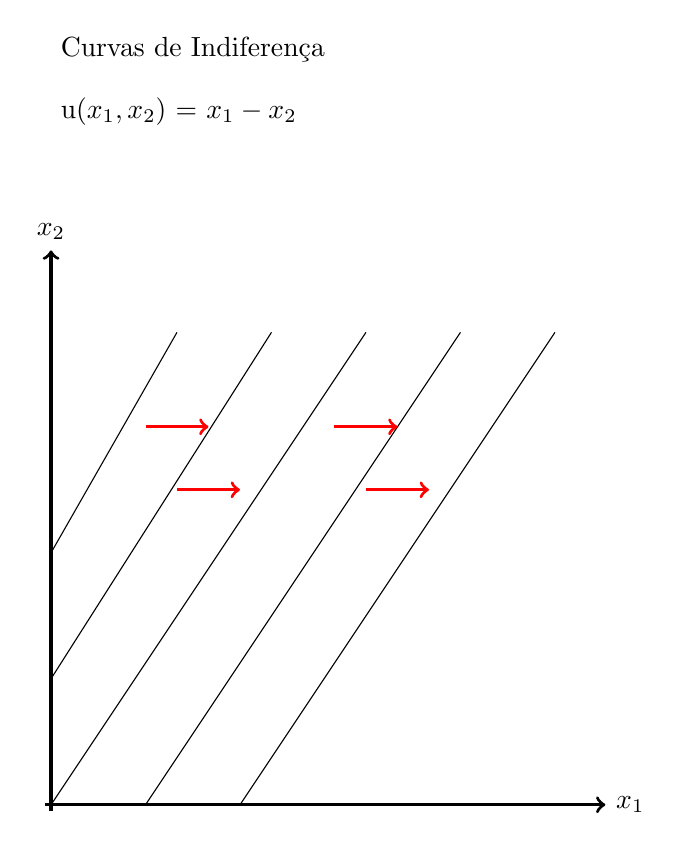
\begin{tikzpicture}[scale=0.8] %Início do desenho e definição da escala
						%Eixos
					\draw[->, very thick] (-0.1,0) -- (8.8,0) node[right]{$x_1$}; %Eixo X1
					\draw[->, very thick] (0,-0.1) -- (0,8.8) node[above]{$x_2$}; %Eixo X2
					
					\draw (0,4) -- (2,7.5);
					\draw (0,2) -- (3.5,7.5);
					\draw (0,0) -- (5,7.5);
					\draw (1.5,0) -- (6.5,7.5);
					\draw (3,0) -- (8,7.5);
                	\draw[->, very thick, red] (1.5,6) -- (2.5,6);
                	\draw[->, very thick, red] (2,5) -- (3,5);
				    \draw[->, very thick, red] (4.5,6) -- (5.5,6);
				    \draw[->, very thick, red] (5,5) -- (6,5);
				    \draw (0,12) node [right] {Curvas de Indiferença};
					\draw (0,11) node [right] {u{$(x_1, x_2)$} = {$x_1 - x_2$}};
					
					
					\end{tikzpicture}\\
				 
			\end{center} 
			
\item[6.] Suponha que uma pessoa esteja consumindo uma cesta de bens tal que a sua utilidade marginal de consumir o bem A é 12 e a sua utilidade marginal de consumir o bem B é 2. Suponha também que os preços dos bens A e B são {$R\$ 2$} e {$R\$ 1$}, respectivamente, e que as preferências desse consumidor são estritamente convexas.\\

\paragraph{} a)Essa pessoa está escolhendo quantidades ótimas dos bens A e B? Caso não esteja, qual bem ela deveria consumir relativamente mais (não se preocupe com a restrição orçamentária nesse item)?\\

\textbf{Resposta:}\\

Suponhamos que os bens consumidos façam parte de uma cesta X qualquer.\\
 \begin{center}
 {$\dfrac{\partial u{(X)}/\partial{x_A}}{\partial u{(X)}/\partial{x_B}}$} = 6 {$\neq$} 2 {$\dfrac{p_A}{p_B}$}\\ 
 
 \end{center}
Como a TMS é maior entre A e B é maior do que a relação dos preços desses itens, o consumidorr pode aumentar sua utilidade se consumir mais do bem bem A e menos do B, pois ele pode optar por trocar duas unidades de B por uma de A, assim sua utilidade aumentará seis vezes mais. \\
 

\paragraph{} b) A sua resposta para o item a) depende do valor da utilidade marginal? Explique.\\

\textbf{Resposta:}\\

Não, depende da relação entre as utilidades marginais, pois independente da função de utilidade usada para representar as preferências ela permanece a mesma.\\


\item[7.] Suponha que Ana consome apenas pão e circo, e suas preferências são bem-comportadas. Um certo dia o preço do pão aumenta e o preço do circo diminui. Ana continua tão feliz quanto antes da mudança de preços (a renda de Ana não mudou).\\

\paragraph{} a) Ana consume mais ou menos pães após a mudança de preços?\\

\textbf{Resposta:}\\

\paragraph{} b) Ana consegue agora comprar a cesta que comprava antes?\\

\textbf{Resposta:}\\

\newpage

\begin{center}
\textbf{Exercícios Problema do Consumidor}\\
\end{center}

\item[1.]  Suponha que existam apenas 2 bens e que a utilidade de um certo indivíduo é u{$(x_1, x_2)$} = {$x_{1}^{0,25} + x_{2}^{0,25}$}\\

\paragraph{} a) Monte o problema do consumidor e derive as demandas ótimas usando o método de
Lagrange.\\

\textbf{Resposta:}\\

\paragraph{} b) Verifique as condições de segunda ordem.\\

\textbf{Resposta:}\\

\paragraph{} c) Mostre que as funções de demanda satisfazem a propriedade de “adding-up”, ou seja,
que {$p_1x_1(p_1, p_2, m) + p_2x_2(p_1, p_2, m)$} é de fato igual a m.\\

\textbf{Resposta:}\\

\paragraph{} d) Mostre que as funções de demanda satisfazem a propriedade de homogeneidade.\\

\textbf{Resposta:}\\

\item[2.] Suponha uma função de utilidade definida por:
\begin{center}
u{$(x_1, x_2)$} = min{$\{x_2 + 2x_1, x_1 + 2x_2\}$}\\
\end{center}

\paragraph{} a) Desenhe a curva de indiferença para u{$(x_1, x_2)$} = 20.\\

\textbf{Resposta:}\\

\paragraph{} b)  Para que valores de {$p_1/p_2$} a solução ótima consistirá em {$x_1 = 0$} e {$x_2 = m/p_2$}?\\

\textbf{Resposta:}\\

\paragraph{} c) Para que valores de {$p_1/p_2$} a solução ótima consistirá em {$x_1 = m/p_1$} e {$x_2 = 0$}?\\

\textbf{Resposta:}\\

\paragraph{} d) Para que valores de {$p_1/p_2$} a solução ótima será interior (ou seja, {$x_{1}^{*} > 0$} e {$x_{2}^{*} > 0$})?\\

\textbf{Resposta:}\\

\item[3.] Considere a utilidade u{$(x_1, x_2) = \sqrt{ax_1 + bx_2}$}.\\

\paragraph{} a)  Calcule a TMS entre os dois bens. Desenhe o mapa de indiferença desta utilidade.\\

\textbf{Resposta:}\\

O mapa de indiferença desta utilidade tem o mesmo formato que mapa de indiferença para a utilidade
u{$(x_1, x_2)$} = {$ax_1 + bx_2$}. Dessa forma, essa utilidade representa bens substitutos perfeitos.

\begin{center} %Centralização do gráfico a ser desenhado
				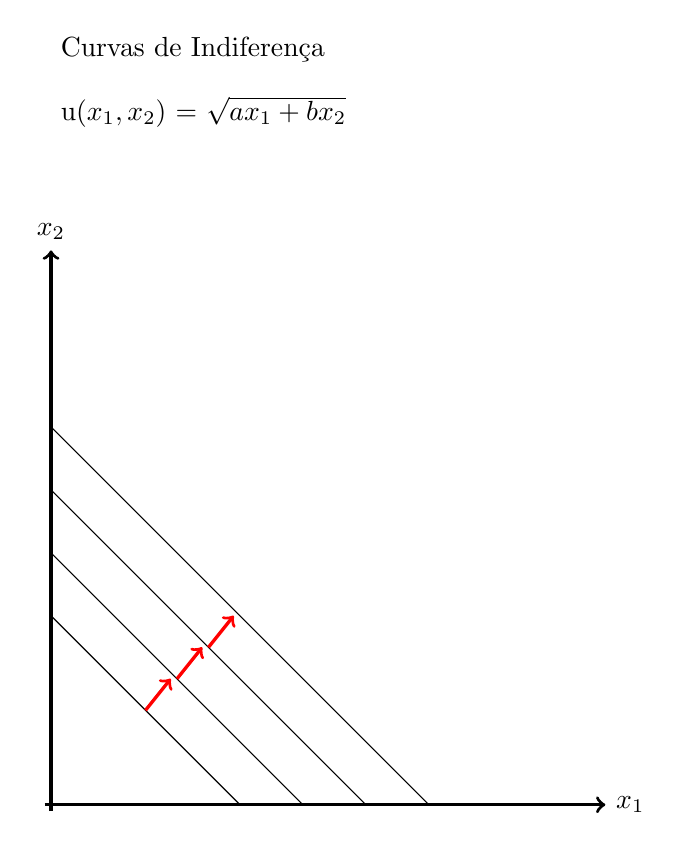
\begin{tikzpicture}[scale=0.8] %Início do desenho e definição da escala
						%Eixos
					\draw[->, very thick] (-0.1,0) -- (8.8,0) node[right]{$x_1$}; %Eixo X1
					\draw[->, very thick] (0,-0.1) -- (0,8.8) node[above]{$x_2$}; %Eixo X2
						%Retas
					\draw (0,6) -- (6,0);
					\draw (0,5) -- (5,0);
					\draw (0,4) -- (4,0);
					\draw (0,3) -- (3,0);
					\draw (0,12) node [right] {Curvas de Indiferença};
					\draw (0,11) node [right] {u{$(x_1,x_2)$} = {$\sqrt{ax_1 + bx_2}$}};
					\draw[->, very thick, red] (1.5,1.5) -- (1.9,2); 
					\draw[->, very thick, red] (2,2) -- (2.4,2.5);
			        \draw[->, very thick, red] (2.5,2.5) -- (2.9,3);
					
				\end{tikzpicture}\\
				 
			\end{center} 

A TMS é igual a -{$\dfrac{a}{b}$}. 

\paragraph{} b) Encontre as funções de demandas ótimas do consumidor. Justifique sua resposta.\\

\textbf{Resposta:} O maior problema do consumidor é atingir o mais alto nível de utilidade, de acordo com sua restrição orçamentária. Como os bens são perfeitamente substitutos, ele escolherá o que tiver o preço menor proporcional. As funções de demanda serão:\\

\begin{center}

{$x_{1}^{M}$}{$(p_1, p_2, m)$} = 
$\begin{cases} m/p_1\textrm{, se } p_1/a < p_2/b\\
               0    \textrm{, se } p_1/a > p_2/b
\end{cases}$\\



e\\


{$x_{2}^{M}$}{$(p_1, p_2, m)$} = 
$\begin{cases}  0     \textrm{, se } p_1/a < p_2/b \\
                m/p_2 \textrm{, se } p_1/a > p_2/b
              
\end{cases}$\\

\end{center}

No caso em que {$p_1/a = p_2/b$} o consumidor será indiferente entre qual bem comprar, pois a TMS sempre será igual a relação dos preços.  consumidor comprará qualquer cesta {$(x_{1}^{*},x_{2}^{*})$} que satisfaça a sua restrição orçamentária {$px_{1}^{*} + px_{2}^{*} = m$}.\\


\paragraph{} c) Agora suponha que a = b = 1 e {$p_1$} = 1, {$p_2$} = 2, m = 100. Ilustre graficamente a solução neste caso. Qual a taxa marginal de substituição na cesta ótima? Para este caso, vale a condição de igualdade de TMS e relação de preços? Discuta intuitivamente sua resposta.\\

\textbf{Resposta:}\\

\begin{center} %Centralização do gráfico a ser desenhado
				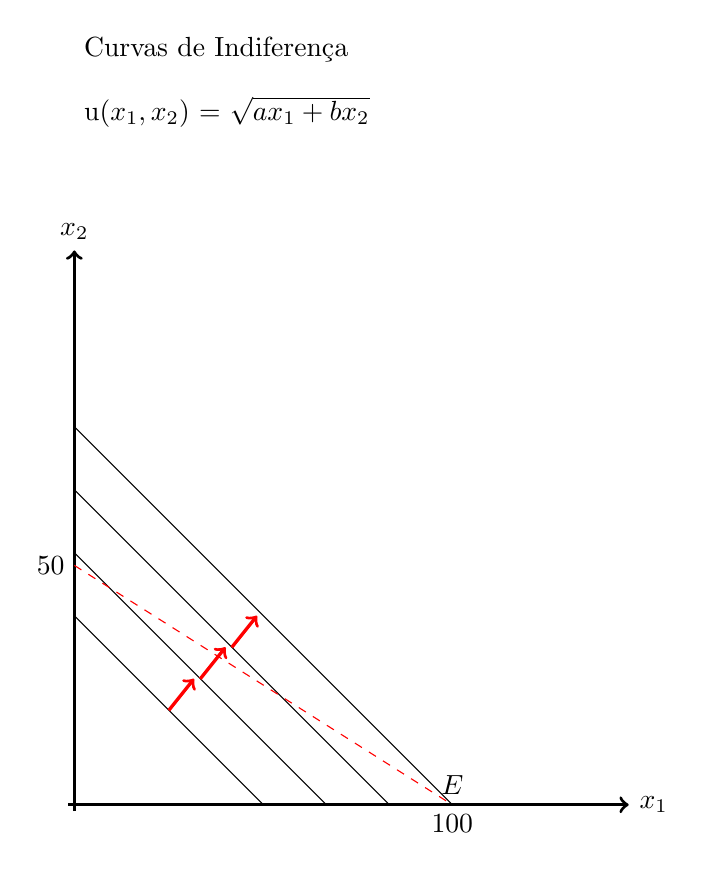
\begin{tikzpicture}[scale=0.8] %Início do desenho e definição da escala
						%Eixos
					\draw[->, very thick] (-0.1,0) -- (8.8,0) node[right]{$x_1$}; %Eixo X1
					\draw[->, very thick] (0,-0.1) -- (0,8.8) node[above]{$x_2$}; %Eixo X2
						%Retas
					\draw (0,6) -- (6,0);
					\draw (0,5) -- (5,0);
					\draw (0,4) -- (4,0);
					\draw (0,3) -- (3,0);
					\draw [dashed,red] (0,3.8) -- (6,0);
					\draw (0,12) node [right] {Curvas de Indiferença};
					\draw (0,11) node [right] {u{$(x_1,x_2)$} = {$\sqrt{ax_1 + bx_2}$}};
					\draw[->, very thick, red] (1.5,1.5) -- (1.9,2); 
					\draw[->, very thick, red] (2,2) -- (2.4,2.5);
			        \draw[->, very thick, red] (2.5,2.5) -- (2.9,3);
			        \node[left] at (0,3.8) {$50$};
			        \node[below] at (6,0) {$100$}; 
			        \node[above] at (6,0) {$E$};
					
				\end{tikzpicture}\\
				 
			\end{center} 
			
TMS = -1/2. Na cesta ótima {$x_{1}^{*} = 100$} e {$x_{2}^{*} = 0$}, não é a válida a igualdade entre a TMS e a relação de preço. Isto ocorre porque estamos em uma solução de canto: apenas o bem 1 é consumido. Se fosse possível, o indivíduo continuaria a trocar bem 2 por bem 1, mas ele já está no limite, sem mais nenhuma quantidade de bem 2 para troca.


\item[4.] Considere a utilidade u{$(x_1, x_2)$} = {$(min\{ax_1, bx_2\})^{2}$}.\\

\paragraph{} a)  Desenhe o mapa de indiferença desta utilidade. Calcule a TMS entre os dois bens.

\textbf{Resposta:}\\

\paragraph{} b) Encontre as funções de demandas ótimas do consumidor. Justifique sua resposta.\\

\textbf{Resposta:}\\

\paragraph{} c) Agora suponha que a = b = 1 e {$p_1$} = 1, {$p_2$} = 2, m = 100. Calcule e ilustre graficamente a solução neste caso. Suponha agora que os preços mudaram para {$p_1$} = 2 e {$p_2$} = 1, e que a renda não se modificou. Calcule e ilustre graficamente a solução neste caso. Compare as duas soluções encontradas neste item. Discuta intuitivamente sua resposta.\\

\textbf{Resposta:}\\

\item[5.] Encontre as demandas ótimas para os seguintes casos, onde {$\alpha > 0$} e {$\beta > 0$}:\\

\paragraph{} a) u{$(x_1, x_2) = x^\alpha_1 x^\beta_2$};\\

\textbf{Resposta:}\\

\paragraph{} b) u{$(x_{1},x_{2})$} = {$x_{1}^{\frac{\alpha}{\alpha + \beta}}$}{$x_{2}^{\frac{\beta}{\alpha + \beta}}$};\\

\textbf{Resposta:}\\

\paragraph{} c) u{$(x_1, x_2)$} = {$\alpha ln(x_1)$} + {$\beta ln(x_2)$}; \\

\textbf{Resposta:}\\

As CPOs resultam em:

\begin{center}

{$(x_1)$}: {$\lambda^{*}p_{1} = \dfrac{\alpha}{x_{1}}$}
\\

{$(x_2)$}: {$\lambda^{*}p_{2} = \dfrac{\beta}{x_{2}}$}
\\

{$(\lambda)$}: m = {$p_{1}x_{1}+p_{2}x_{2}$}

\end{center}

Dividindo a primeira CPO pela segunda CPO, obtemos:

\begin{center}

{$\dfrac{\alpha x_{2}}{\beta x_{1}}$} = {$\dfrac{p_{1}}{p_{2}}$} {$\Rightarrow$} {$x_2 =\dfrac{p_1}{p_2}\left[\dfrac{\beta x_{1}}{\alpha}\right]$}\\

\end{center}

Substituimos agora essa expressão para {$x_2$} na reta orçamentária (terceira CPO):\\

\begin{center}

m = {$p_{1}x_{1}+p_{2} \left(\dfrac{p_1}{p_2}\left[\dfrac{\beta x_{1}}{\alpha}\right]\right)$}
{$\Rightarrow$} {$\dfrac{\alpha}{\alpha + \beta}$} {$\left(\dfrac{m}{p_1}\right)$}\\

\end{center}

Substituindo {$x_1$} de volta em {$x_2$}, obtemos as duas funções de demanda:\\

\begin{center}

{$x_1(p_1,p_2,m) = \dfrac{\alpha}{\alpha + \beta} \left(\dfrac{m}{p_1}\right)$} e {$x_2(p_1,p_2,m) = \dfrac{\beta}{\alpha + \beta} \left(\dfrac{m}{p_2}\right)$}

\end{center}

Qual a relação entre as demandas encontradas acima? Justifique a sua resposta. Com base
na sua resposta, se a utilidade é do tipo u{$(x_1, x_2)$} = {$x^\alpha_1 x^\beta_2$}, é possível tranformá-la em uma utilidade do tipo u{$(x_1, x_2)$} = {$x_{1}^{\gamma}x_{2}^{1-\gamma}$}, com {$0 < \gamma < 1$}? Se sim, qual a relação entre {$\alpha$}, {$\beta$} e {$\gamma$}?\\


\textbf{Resposta:}\\

\item[6.] Calcule as demandas de um consumidor representado por uma utilidade CES (elasticidade
de substituição constante) dada por:\\

\begin{center}
u{$(x_1, x_2)$} = {$[ax_{1}^{\rho} + bx_{2}^{\rho}]^\frac{1}{\rho}$},   {$0\neq \rho < 1$}.\\
\end{center}

\newpage

\begin{center}
\textbf{Exercícios Utilidade Indireta e Demanda}\\
\end{center}

\item[1.] Considere a seguinte função de utilidade:\\

\begin{center}
u{$(x_1, x_2)$} = {$x_{1}^{0,5} + x_{2}^{0,5}$}.\\
\end{center}

\paragraph{} a) Determine as funções de demanda marshallianas e a função de utilidade indireta.\\

\textbf{Resposta:}\\

\paragraph{} b) Mostre que a função de utilidade indireta satisfaz a propriedades de homogeneidade de
grau 0 nos preços e na renda.\\

\textbf{Resposta:}\\

\item[2.] Suponha que a utilidade de Bernardo seja u{$(x_1, x_2)$} = min{$\{x_1, x_2\}$}. Suponha que os preços do bem 1 e do 2 sejam {$p_1 = R\$ $} 1,00 e {$p_2 = R\$ $} 1,00 e que a renda de Bernardo seja R\$ 120.

\paragraph{} a) Quais são as quantidades consumidas de cada bem por Bernardo? Qual a utilidade que
ele obtém?\\

\textbf{Resposta:}\\

{$p_1$ = R\$ 1,00};\\
{$p_2$ = R\$ 1,00};\\
m = R\$ 120;\\

{$\begin{cases} x_{1} = x_{2}\\
p_{1}x_{1}+p_{2}x_{2}=m
\end{cases}$}\\


{$1x_{1}+1x_{2} = 120$}\\
{$1x_{1}+1(x_{1}) = 120$}\\
{$x_1(1+1) = 120$}\\
{$x_1 = 120/(1+1)$} {$\rightarrow$} {$x_{1} = 60$}\\
como {$x_{1}^{*} = x_{2}^{*} = 60$} e a utilidade é {$U^{*} = 60$}


\paragraph{} b) Se o governo instituir um imposto sobre o consumo do bem 1 de modo que o seu preço
aumente para {$p_1 = R\$ $} 2, quais serão as quantidades consumidas por Bernardo dos dois bens? Qual a utilidade de Bernardo agora?\\

\textbf{Resposta:}\\

{$p_1$ = R\$ 2,00};\\
{$p_2$ = R\$ 1,00};\\
m = R\$ 120;\\

{$\begin{cases} x_{1} = x_{2}\\
p_{1}x_{1}+p_{2}x_{2}=m
\end{cases}$}\\



{$2x_{1}+1x_{2} = 120$}\\
{$2x_{1}+1(x_{1}) = 120$}\\
{$x_1(2+1) = 120$}\\
{$x_1 = 120/(2+1)$} {$\rightarrow$} {$x_{1} = 40$}\\
como {$x_{1}^{*} = x_{2}^{*} = 40$} e a utilidade é {$U^{*} = 40$}


\paragraph{} c) Suponha que o governo abandone a ideia do imposto sobre o consumo do bem 1 e decida
taxar a renda do consumidor por um valor que resulte no mesmo montante que obteria com o imposto descrito no item anterior. Quais as novas quantidades consumidas dos dois bens? Qual a utilidade de Bernardo agora?

\textbf{Resposta:}\\

Considerando o novo valor pelo item anterior, serão vendidas 40 unidades do bem 1. O governo então arrecadará R\$ 40 de IR. Retirando o imposto de R\$ 40,00 da renda inicial, R\$ 120,00 obtemos a nova renda de R\$ 80,00 como mostra abaixo:\\

{$\begin{cases} \overline{m} = m-tx_{1}\\
\overline{m} = 120-40(1)\\
\overline{m} = 80
\end{cases}$}\\

{$x_{1}=x_{2}\\
1x_{1}+1x_{2} = 80\\
x_{1} = (1+1) = 80
x_1 = 80/(1+1) = 40$}\\
{$x_{1}^{*} = x_{2}^{*} = 40$} e a {$u^{*} = 40$}\\


\paragraph{} d) Explique intuitivamente a razão do princípio Lump Sum neste exemplo não resulta numa
utilidade maior para Bernardo no caso do imposto de renda do que no caso do imposto sobre o consumo.\\

\textbf{Resposta:}\\

Como a utilidade é do tipo Leontief, os bens devem ser consumidos em proporçoes fixas. Logo, ao substituir os imposto sobre o consumo pelo imposto sobre a renda, o consumidor continuará consumindo as mesmas quantidades dos dois bens, pois não há possibilidade de substituição. Dessa forma, os dois tipos de impostos levam ao mesmo nivel de bem-estar. 

\item[3.] Suponha que a utilidade de Ana seja u{$(x_1, x_2)$} = {$x_1x_2$}. Suponha que os preços do bem 1 e do 2 sejam {$p_1 = R\$ $} 2 e {$p_2 = R\$ $} 2 e que a renda de Ana seja R\$ 600.\\

\textbf{Resposta:}\\

\paragraph{} a) Quais são as quantidades consumidas de cada bem por Ana? Qual a utilidade que ela
obtém?\\

\textbf{Resposta:}\\

\paragraph{} b) Se o governo instituir um subsídio sobre o consumo do bem 1 de modo que o seu preço
diminua para {$p_1 = R\$ $} 1, quais ser˜ao as quantidades consumidas por Ana dos dois bens? Qual a utilidade de Ana agora?\\

\textbf{Resposta:}\\

\paragraph{} c) Suponha que o governo abandone a ideia do subsídio sobre o consumo do bem 1 e decida
repassar um montante fixo para Ana de modo que resulte no mesmo gasto para o governo que o esquema de subsídio anterior gerava. Quais as novas quantidades consumidas dos dois bens? Qual a utilidade de Ana agora?\\

\textbf{Resposta:}\\

\paragraph{} d) Usando a intuição econômica, elabore um argumento a favor de programas de transferência de renda como o Programa Bolsa Família sobre programas do tipo Vale Gás, que subsidiava o preço do gás de cozinha para pessoas carentes. Faça o raciocínio inverso: discuta as vantagens, caso existam, de um programa de subsídios para o consumo de certos bens sobre um programa de transferência de renda.\\

\textsc{\textbf{Resposta:}\\}

\item[4.] Suponha que a utilidade de Rafael seja u{$(x_1, x_2)$} = {$x_{1}^{0,2}x_{2}^{0,8}$}, onde {$x_1$} é a quantidade de alimentos que Rafael consome e {$x_2$} é a quantidade de todos os outros bens que Rafael consome (um bem composto, portanto). Suponha que o preço do bem 2 é {$p_2$} = R\$ 1 e que a renda de Rafael  R\$ 1000.\\

\paragraph{} a) Se o preço do bem 1 é R\$ 2, qual é o consumo de alimentos de Rafael?\\

\textbf{Resposta:}\\



\paragraph{} b) Se o preço do bem 1 duplicar, qual será o novo consumo de alimentos de Rafael?\\

\textbf{Resposta:}\\ 
\begin{center}
L = {$(x_{1}^{0,2}x_{2}^{0,8} - p_{1}x_{1}\lambda - p_{2}x_{2}\lambda + 1000\lambda = 0)$}
\end{center}

f'{$(x_{1}) = 0,2x_{1}^{-0,8}x_{2}^{0,8} - p_{1}\lambda = 0 \Longrightarrow \lambda = \dfrac{0,2x_{2}^{0,8}}{p_{1}x_{1}^{0,8}}$} \\

f'{$(x_{2}) = 0,8x_{1}^{0,2}x_{2}^{-0,2} - p_{2}\lambda = 0 \Longrightarrow \lambda = \dfrac{0,8x_{1}^{0,2}}{p_{2}x_{2}^{0,2}}$} \\

f'{$(\lambda) = -p_{1}x_{1} - p_{2}x_{2} + m = 0 \Longrightarrow -p_{1}x_{1} - p_{2}x_{2} = - m$}\\

\begin{center}
Igualando {$ \lambda = \lambda$}

\end{center}


\begin{center} 
{$\dfrac{0,2x_{2}^{0,8}}{p_{1}x_{1}^{0,8}}$} = {$\dfrac{0,8x_{1}^{0,2}}{p_{2}x_{2}^{0,2}}$}\\
\end{center}

\begin{center}
{$0,2p_{2}x_{2} = 0,8p_{1}x_{1}$}\\
\end{center}

\begin{center}
{$x_{2} = \dfrac{0,8p_{1}x_{1}}{0,2p_{2}} \rightarrow x_{2} = \dfrac{4p_{1}x_{1}}{p_{2}}$}
\end{center}

\begin{center}
Substituindo {$x_{2}$} na 3ª CPO:\\
\end{center}

\begin{center}
f'{$(\lambda) = -p_{1}x_{1} - p_{2}x_{2} + m = 0$} {$\rightarrow$} {$-p_{1}x_{1} - p_{2}x_{2} = - m$}\\
\end{center}

\begin{center}
{$ - p_{1}x_{1} - p_{2} \left(\dfrac{4p_{1}x_{1}}{p_{2}}\right) = -m$}\\
\end{center}

\begin{center}
{$x_{1} = \dfrac{m}{5p_{1}}$}\\
\end{center}

\begin{center}
Substituindo {$x_{1}$} em {$x_{2}$}\\
\end{center}

\begin{center}
{$x_{2} = \dfrac{4p_{1}{\dfrac{m}{5p_{1}}}}{p_{2}}$} {$\rightarrow$} {$x_{2} = \dfrac{4m}{5p_{2}}$}
\end{center}

\begin{center}
Temos então as funções de demanda dos dois bens:\\
\end{center}

\begin{center}
{$x_{1} = \dfrac{m}{5p_{1}}$} e {$x_{2} = \dfrac{4m}{5p_{2}}$}
\end{center}

\begin{center}
Agora substituindo renda e preços achamos as demandas pelos dois bens: {$x_{1}^{*}$} e {$x_{2}^{*}$}\\
\end{center}

\begin{center}
{$x_{1} = \dfrac{1000}{5(4)}$} e {$x_{2} = \dfrac{4(1000)}{5(1)}$}\\
\end{center}

\begin{center}
{$x_{1}^{*} = 50$} e {$x_{2}^{*} = 800$}
\end{center}



\paragraph{} c) Suponha agora que o governo resolva subsidiar alimentos, mantendo o preço igual a R\$ 2
– ou seja, concendendo um subsídio de R\$ 2 por unidade consumida de {$x_1$}. Se o governo
financia esse subsídio por meio da cobrança de um imposto sobre a renda, qual é o novo nível de consumo de {$x_1$} de Rafael?\\

\textbf{Resposta:}\\

\paragraph{} d) Construa um diagrama comparando as situações em b) e c) e mostre em qual situação o consumidor está melhor.\\

\textbf{Resposta:}\\

\paragraph{} e) Relacione a sua resposta para esta questão com o princípio Lump Sum.\\

\textbf{Resposta:}\\
O subsídio em cima da renda aumenta mais a utilidade do consumidor do que o subsídio em cima do bem.

\newpage

\begin{center}
\textbf{Exercícios Elasticidades}\\
\end{center}


\item[1.] Derive as agregações de Engel e Cournot para o caso de n bens. Reescreva essas agregações
em termos de elasticidades. Interprete (por exemplo, é possível que todos os bens que um indivíduo consuma sejam bens inferiores? Por quê? Se um indivíduo consome n bens, no máximo quantos bens podem ser inferiores? Justifique sua resposta).\\

\textbf{Resposta:}\\

\item[2.] Suponha a existência de n bens. Usando a propriedade de homogeneidade das funções de demanda Marshalliana, mostre que as elasticidades-preço e renda de um dado bem i satisfazem a seguinte igualdade:\\

\begin{center}                                                        
{$\eta_{i}$} + {$\displaystyle \sum_{j=1}^{n} \epsilon_{ij} = 0,$}
\hspace{65mm}(9)
\end{center}

onde {$\eta_{i}$} é a elasticidade-renda do bem {$i$} e {$\epsilon_{ij}$} é a elasticidade-preço da demanda do bem {$i$} com relação ao preço do bem {$j$}. Interprete intuitivamente a relação (9) acima.\\

\textbf{Resposta:}\\

A propriedade de homogeneidade implica que os agentes não sofrem de ilusão monetária. Logo, para cada para cada bem {$i$} = 1, . . . , n, temos:
\begin{center}
{$x_{i}(t{\textbf{p}}, t{m}) = x_{i}(p, m)$}, para todo t {$>$} 0.
\end{center}
 
Podemos derivá-la com relação a t, o que resulta, pela regra da cadeia, em:

\begin{center}
{$\displaystyle \sum_{j=1}^{n}$} {$\dfrac{\partial x_{i}(t \textbf{p}, tm)}{\partial p_{j}}$}{$p_{j}$} +
{$\dfrac{\partial x_{i}(t \textbf{p}, tm)}{\partial m}$}{$m$} = 0
\hspace{30mm}(10)
\end{center}

Dividindo a igualdade acima por {$x_{i}$} {$(t\textbf{p}, tm)$}:\\

{$\dfrac{\partial x_{i}}{\partial p_{j}}$}{$\dfrac{p_{j}}{x_{i}}$} +
{$\dfrac{\partial x_{i}}{\partial m}$}{$\dfrac{m}{x_{i}}$} = 0\\

fazendo t = 1 e reescrevendo (10) em termos de elasticidades obtemos a expressão desejada:

{$\displaystyle \sum_{j=1}^{n}$} {$\epsilon_{ij} + \eta_{i}$} = 0,  para todo {$i$} = 1, ... , n.\\


\item[3.] Suponha que que a elasticidade-renda da demanda per capita de cerveja é constante e igual a 3/4 e a elasticidade-preço é também constante e igual a -1/2. Os consumidores gastam, em média, R\$ 400,00 por ano com cerveja . A renda média anual destes consumidores é R\$ 6.000,00. Cada garrafa de cerveja custa R\$ 3,00.

\paragraph{}a) Se o governo pretende desestimular o consumo de cerveja pela metade, qual deve ser o
aumento no preço da cerveja que alcançaria esta meta?

\textbf{Resposta:}\\

\paragraph{}b) Suponha que o governo estimou um aumento da renda média anual no próximo ano de R\$ 3.000,00. O governo deseja manter o nível de consumo de cerveja constante no próximo ano, usando um imposto sobre o preço da cerveja. Qual deve ser o aumento no preço da cerveja no próximo ano para que o seu consumo n˜ao se modifique, dado que a previs˜ao de aumento de renda se realize?\\

\textbf{Resposta:}\\

\newpage

\begin{center}
\textbf{Exercícios Minimização do Dispêndio}\\
\end{center}

\item[2.] Encontre as demandas Hicksianas e a função dispêndio para os seguintes casos:\\

\paragraph{}a)Utilidade Cobb-Douglas: u{$(x_1, x_2)$} = {$x^{\alpha}_{1}x^{1-\alpha}_{2}$}, {$0<\alpha>1$}.\\

\textbf{Resposta:}\\


O Lagrangeano deste caso é:
L= {$p_{1}x_{1}+p_{2}x_{2}+ \mu (\overline{u} -x_{1}^{\alpha}x_{2}^{1-\alpha})$}\\


As CPOs resultam em:\\

(1ª) f'{$(x_1) = p_{1} - \alpha x_{1}^{\alpha - 1}x_{2}^{1 - \alpha}$}  {$\rightarrow p_{1} = \mu \alpha x_{1}^{\alpha - 1}x_{2}^{1 - \alpha}$}\\


(2ª) f'{$(x_2) = p_{2} - (1 - \alpha) x_{1}^{\alpha}x_{2}^{- \alpha}$}  {$\rightarrow p_{2} = \mu (1 - \alpha) x_{1}^{\alpha}x_{2}^{- \alpha}$}\\


(3ª) f'{$(\mu) = \overline{u} - x_{1}^{\alpha}x_{2}^{1 - \alpha}$}\\



Dividindo a 1ª CPO pela 2ª, encontraremos uma expressão para {$x_{1}$} em função de {$x_{2}$
}\\

{$\dfrac{p_1}{p_2} = \dfrac{\mu \alpha x_{1}^{\alpha - 1}x_{2}^{1 - \alpha}}{\mu (1 - \alpha) x_{1}^{\alpha}x_{2}^{- \alpha}}$} {$\rightarrow \dfrac{p_1}{p_2} = \dfrac{\alpha}{(1- \alpha)} \dfrac{x_1}{x_2}$} {$\rightarrow x_{1} = \dfrac{\alpha}{(1 - \alpha)}\dfrac{p_2}{p_1} x_{2}$}\\


Substituindo a expressão encontrada acima na 3ª CPO, encontraremos a demanda para o bem 2:

{$\overline{u} = \left(\dfrac{\alpha}{(1 - \alpha)}\dfrac{p_{2}}{p_{1}}x_{2}\right)^{\alpha}x_{2}^{1 - \alpha}$}
{$\Longrightarrow \left(\dfrac{\alpha}{(1 - \alpha)}\right)\left(\dfrac{p_2}{p_1}\right)^{\alpha}x_{2}^{\alpha}x_{2}^{1-\alpha}$}\\


{$x_{2} = \dfrac{\overline{u}}{\left(\dfrac{\alpha}{(1-\alpha)}\dfrac{p_2}{p_1}\right)^{\alpha}}$}
{$\Longrightarrow \dfrac{\overline{u}}{\left(\dfrac{\alpha}{(1-\alpha)}\right)^{\alpha}\left(\dfrac{p_2}{p_1}\right)^{\alpha}}$}\\ 


{$x_{2}\left\lbrace = \overline{u} \left(\dfrac{\alpha}{(1 - \alpha)}\right)^{-\alpha}p_{1}^{\alpha}p_{2}^{-\alpha}\right\rbrace$}\\

Substituindo a demanda do bem 2 na expressão de {$x_{1}$} em funcão de {$x_{2}$}, encontramos
a demanda do bem 1. 

{$x_{1} = \dfrac{\alpha}{(1 - \alpha)}\dfrac{p_2}{p_1} x_{2}$}\\


{$x_{1} = \dfrac{\alpha}{(1 - \alpha)}\dfrac{p_2}{p_1}\left(\overline{u} \left(\dfrac{\alpha}{(1 - \alpha)}\right)^{-\alpha}p_{1}^{\alpha}p_{2}^{-\alpha}\right)$}\\

{$x_{1} = \left\lbrace\left(\dfrac{\alpha}{(1 - \alpha)}\right)^{1 - \alpha}p_{1}^{\alpha - 1}p_{2}^{1 - \alpha}\overline{u}\right\rbrace$}\\

A função de dispêndio é encontrada substituindo as demandas compensadas no gasto do consumidor: e{$(p_1, p_2, \overline{u}) = p_{1}x_{1}^{h} +  p_{2}x_{2}^{h}$}. Simplificando essa expressão, obtemos:

{$p_{1}\left(\left(\dfrac{\alpha}{(1 - \alpha)}\right)^{1 - \alpha}p_{1}^{\alpha - 1}p_{2}^{1 - \alpha}\overline{u}\right) + p_{2}x_{2}\left(= \overline{u} \left(\dfrac{\alpha}{(1 - \alpha)}\right)^{-\alpha}p_{1}^{\alpha}p_{2}^{-\alpha}\right)$}\\

{$e(p_{1}, p_{2},\overline{u}) = \alpha^{-\alpha}(1 - \alpha)^{\alpha - 1}p_{1}^{\alpha}p_{2}^{1 - \alpha} \overline{u}$}\\


\paragraph{}b) Utilidade linear: u{$(x_1, x_2)$} = {$ax_{1}+bx_{2}$}, {$a,b>0$}.\\

\textbf{Resposta:}\\

{$min_{x_{1}, x_{2} \geq 0}$} {$p_{1}x_{1} + p_{2}x_{2}$} s.a {$ax_{1}+bx_{2} = \overline{u}$}\\

O consumidor irá consumir o bem relativamente mais barato, em uma quantidade que assegure a ele o nível de utilidade {$\overline{u}$}, portanto, as demandas Hicksianas são:

{$x_{1}^{h}(p_{1},p_{2}$}, {$\overline{u})$} = 
{$\begin{cases} \overline{u}/a\textrm{, se } p_1/a < p_2/b\\
0\textrm{, se } p_1/a > p_2/b
\end{cases}$} 

e

{$x_{2}^{h}(p_{1},p_{2}$}, {$\overline{u})$} = 
{$\begin{cases} \overline{u}/b\textrm{, se } p_1/a > p_2/b\\
0\textrm{, se } p_1/a < p_2/b
\end{cases}$} 
\\

No caso em que {$p_1/a = p_2/b$}, o consumidor comprará qualquer cesta {$(x_{1}^{*},x_{2}^{*})$} tal que satisfaça a restrição, {$ax^{*}_{1} + bx_{2}^{*} = \overline{u}$}. A função dispêndio é:
\\

{$e(p_{1},p_{2}$}, {$\overline{u})$} = 
{$\begin{cases} p_{1}(\overline{u}/a)\textrm{, se } p_1/a \leq p_2/b\\
p_{2}(\overline{u}/b)\textrm{, se } p_1/a > p_2/b\\
p_{1}(\overline{u}/a) = p_{2}(\overline{u}/b)\textrm{, se } p_1/a = p_2/b
\end{cases}$} 
\\

De modo mais simples, a função dispêndio é: 

{$e(p_{1}, p_{2}, \overline{u}) = p_{1}x^{h}_{1}+ p_{2}x^{h}_{2} = min \left\lbrace\dfrac{p_1}{a}\overline{u}, \dfrac{p_{2}}{b} \overline{u} \right\rbrace$} = min{$\left\lbrace\dfrac{p_1}{a}, \dfrac{p_{2}}{b}\right\rbrace \overline{u}$}\\


\paragraph{}c) Utilidade Leontief: u{$(x_1, x_2)$} = min{$\{ax_1, bx_2\}$}, {$a, b > 0$}.\\

\textbf{Resposta:}\\

{$min_{{x_{1}, x_{2} \geq 0}}$} {$p_{1}x_{1} + p_{2}x_{2}$} s.a {$\{ax_{1},bx_{2}\} = \overline{u}$}

Vimos que dois bens são complementares perfeitos se são consumidos conjuntamente, em proporções fixas. Logo, as demandas Hicksianas são:\\


{$x^{h}_{1}(p_1, p_2, \overline{u}) = \dfrac{\overline{u}}{a}$}
e 
{$x^{h}_{2}(p_1, p_2, \overline{u}) = \dfrac{\overline{u}}{b}$}

A função dispêndio é: 

{$e(p_{1}, p_{2}, \overline{u})$} = {$p_{1}x^{h}_{1}+ p_{2}x^{h}_{2}$} = {$p_{1}\dfrac{\overline{u}}{a}$} + {$p_{2} \dfrac{\overline{u}}{b}$} = {$\left(\dfrac{p_1}{a} + \dfrac{p_2}{b}\right)\overline{u}$}



\paragraph{}d) Utilidade CES: u{$(x_1, x_2)$} = {$[ax^{\rho}_{1}+bx^{\rho}_{2}]^\frac{1}{\rho}$}, {$a,b > 0, \rho < 1, \rho \neq 0$}. \\

\textbf{Resposta:}\\

{$L = p_{1}x_{1} + p_{2}x{2} + \mu (\overline{u}- [ax_{1}^{\rho} + bx_{2}^{\rho}]^{1/\rho})$}\\

As CPOs resultam em:

(1ª)f'{$(x_{1})$} = {$p_{1} - \dfrac{1}{\rho}$} {$(ax_{1}^{\rho}+bx_{2}^{\rho})^{\frac{1}{\rho}- 1} \rho ax_{1}^{\rho - 1} \mu$} {$\Rightarrow p_{1} = \mu[ax_{1}^{\rho} + bx_{2}^{\rho}]^{\frac{1}{\rho} - 1}ax_{1}^{\rho - 1}$}\\

(2ª)f'{$(x_{2})$} = {$p_{2} - \dfrac{1}{\rho}$} {$(ax_{1}^{\rho}+bx_{2}^{\rho})^{\frac{1}{\rho}- 1} \rho bx_{1}^{\rho - 1} \mu$} {$\Rightarrow p_{1} = \mu[ax_{1}^{\rho} + bx_{2}^{\rho}]^{\frac{1}{\rho} - 1}bx_{1}^{\rho - 1}$}\\

(3ª)f'{$(\mu) = \overline{u} - [ax_{1}^{\rho} + bx_{2}^{\rho}]^{\frac{1}{\rho}}$}\\

Dividindo as duas primeiras CPOs, achamos uma expressão para {$x_{2}$} em função de {$x_{1}$}\\

{$\dfrac{p_{1}}{p_{2}} = \dfrac{\mu[ax_{1}^{\rho} + bx_{2}^{\rho}]^{\frac{1}{\rho}-1}ax_{1}^{\rho-1}}{\mu[ax_{1}^{\rho} + bx_{2}^{\rho}]^{\frac{1}{\rho}-1}bx_{1}^{\rho-1}}$}\\

{$\dfrac{p_{1}}{p_{2}}$}{$\dfrac{ax{1}^{\rho - 1}}{bx_{2}^{\rho - 1}}$} {$\Rightarrow$} 
{$x_{2} =  \left(\dfrac{ap_{2}}{bp_{1}}\right)^{1/\rho-1}x_{1}$}\\

Substituindo essa expressão na terceira CPO, encontramos a demanda Hicksiana para o bem 1:

{$\overline{u} - [ax_{1}^{\rho} + b\left(\dfrac{ap_{2}}{bp_{1}}\right)^{\frac{1}{\rho-1}}x_{1}                   ^{\rho}]^{\frac{1}{\rho}}$}\\



{$x_{1}$} = {$\left[a + b\left(\dfrac{ap_{2}}{bp_{1}}\right)^{\frac{\rho}{\rho-1}} \right]^{-\frac{1}{\rho}}\overline{u}$}\\

Substituindo a demanda do bem 1 na expressão de {$x_2$} em funçãao de {$x_1$},encontramos a demanda Hicksiana do bem 2: 


{$x_{2} =  \left(\dfrac{ap_{2}}{bp_{1}}\right)^{\frac{1}{\rho-1}}\left[\left(a + b\left(\dfrac{ap_{2}}{bp_{1}}\right)^{\frac{\rho}{\rho-1}} \right)^{-\frac{1}{\rho}}\overline{u}\right]$}\\

A função de dispêndio é:\\
{$e(p_1, p_2, \overline{u})$} = {$p_{1}\left(\left[a + b\left(\dfrac{ap_{2}}{bp_{1}}\right)^{\frac{\rho}{\rho-1}} \right]^{-\frac{1}{\rho}}\overline{u}\right)$} + {$p_{2}\left(\left(\dfrac{ap_{2}}{bp_{1}}\right)^{\frac{1}{\rho-1}}\left[\left(a + b\left(\dfrac{ap_{2}}{bp_{1}}\right)^{\frac{\rho}{\rho-1}} \right)^{-\frac{1}{\rho}}\overline{u}\right]\right)$}\\


\newpage

\begin{center}
\textbf{Exercícios Dualidade}\\
\end{center}


\item[2.] A utilidade de Carlos é u{$(x_{1}, x_{2})$} = min{$\{x_{1}, x_{2}\}$}. A renda de Carlos é R\$20, e os preços dos bens 1 e 2 são R\$1 e R\$1. Suponha que o preço do bem 1 aumentou para R\$2.



\paragraph{} a) Encontre o efeito total desse aumento na demanda de Carlos pelo bem 1.\\

\textbf{Resposta:}\\

{$m = R\$ 20,00; p_{1} = 1,00; p_{2} = 1,00$}\\

u{$(x_{1}, x_{2})$} = min{$\{x_{1}, x_{2}\}$}\\

{$\begin{cases} x_{1} = x_{2}\\
p_{1}x_{1}+p_{2}x_{2} = m \Rightarrow
x_{1}^{M} = x_{2}^{M} = 10
\end{cases}$} 

{$\begin{cases} x_{1} = x_{2}\\
p_{1}x_{1}+p_{2}x_{2} = m \Rightarrow
\hat{x}_{1}^{M} = \hat{x}_{2}^{M} = 20/3 \cong 6,66
\end{cases}$}


Com os preços antigos, Carlos, demandava 10 unidades de cada bem. Já com os preços novos a demanda é de 20/3. O Efeito Total desse aumento na demanda de Carlos  pelo bem 1 é a redução no consumo desse bem, ficando igual a {$10 - 20/3 = 3.33$}.


\paragraph{} b) Decomponha o efeito total em efeito substituição Hicksiano e efeito renda. Interprete
intuitivamente o seu resultado.\\

\textbf{Resposta:}\\

Na utilidade Leontief, não há possibilidade de substituição, pois os bens são complementares perfeitos. Logo o efeito substituição é nulo e o efeito total é efeito renda. Como mostra o gráfico:

\begin{center} %Centralização do gráfico a ser desenhado
				\begin{tikzpicture}[scale=0.8] %Início do desenho e definição da escala
						%Eixos
					\draw[->, very thick] (-0.1,0) -- (9.8,0) node[right]{$x_1$}; %Eixo X1
					\draw[->, very thick] (0,-0.1) -- (0,8.8) node[above]{$x_2$}; %Eixo X2
					
						%Curvas
					\draw (2.5,3) -- (7,3);
					\draw (2.5,3) -- (2.5,7);
					\draw (2.9,3) node [above]{{$\hat{E}$}};
					\draw (9,9) node [above] {Preço do bem 1 aumentou};
					\draw (9,8) node [above] {Efeito substituição é nulo};
					\draw (9,7) node [above] {Efeito Total = Efeito Renda};
				
				    \draw (3.5,4) -- (7,4);
					\draw (3.5,4) -- (3.5,7);
					\draw (3.8,4.2) node [above]{{${E}$}};
					
		                %Retas
		            \draw (0,7) -- (4.4,0);
		            \draw (0,7) -- (8.2,0);
		            \node[left] at (0,7){$\dfrac{m}{p_{2}}$};
		            \node[below] at (4.4,0){$\dfrac{m}{p'_{1}}$};
		            \node[below] at (8.2,0){$\dfrac{m}{p_{1}}$};
				\end{tikzpicture}\\
			\end{center} 

\paragraph{}c) Decomponha o efeito total em efeito substituição de Slutsky e efeito renda. Interprete
intuitivamente o seu resultado.\\


\textbf{Resposta:} Para o caso de um efeito de substituição de Slutsky, a compensação é de modo que
o consumidor possa comprar a mesma cesta que adquiria aos preços antigos, mas agora aos preços novos. Portanto, o efeito substituição de Slutsky vai também ser zero e o efeito total é todo efeito renda.\\


\begin{center} %Centralização do gráfico a ser desenhado
				\begin{tikzpicture}[scale=0.8] %Início do desenho e definição da escala
						%Eixos
					\draw[->, very thick] (-0.1,0) -- (9.8,0) node[right]{$x_1$}; %Eixo X1
					\draw[->, very thick] (0,-0.1) -- (0,8.8) node[above]{$x_2$}; %Eixo X2
					
						%Curvas
					\draw (2.5,3) -- (7,3);
					\draw (2.5,3) -- (2.5,7);
					\draw (2.9,3) node [above]{{$\hat{E}$}};
					\draw (9,9) node [above] {Preço do bem 1 aumentou};
					\draw (9,8) node [above] {Efeito substituição de Slutsky = nulo};
					\draw (9,7) node [above] {Efeito Total = Efeito Renda};
				    \draw (3.5,4) -- (7,4);
					\draw (3.5,4) -- (3.5,7);
					\draw (3.8,4.2) node [above]{{${E}$}};
					
		                %Retas
		            \draw (0,7) -- (4.4,0);
		            \draw (0,7) -- (8.2,0);
		            \node[left] at (0,7){$\dfrac{m}{p_{2}}$};
		            \draw[dashed] (4.7,3) -- (4.7,0); %Pontilhado eixo X1
                    \draw[dashed] (4.7,3) -- (0,3); %Pontilhado eixo X2
                    \draw[dashed] (2.5,3) -- (0,3); %Pontilhado eixo X1
                    \draw[dashed] (3.5,4) -- (3.5,0); %Pontilhado eixo X2
                    \draw[dashed] (3.5,4) -- (0,4); %Pontilhado eixo X1
                    \draw[dashed] (2.5,3) -- (2.5,0); %Pontilhado eixo X2
		            \node[below] at (4.7,0){$x'''_{1}$};
		            \node[below] at (2.5,0){$x''_{1}$};
		            \node[below] at (3.5,0){$x'_{1}$};
		            \node[left] at (0,3){$x''_{2} \textrm{ e } x'''_{2}$};
		            \node[left] at (0,4){$x'_{2}$};
				\end{tikzpicture}\\
			\end{center} 


\item[4.] Suponha que a função utilidade indireta de um consumidor é:\\

\begin{center}
{$ v(p_1, p_2, m) = 50 \left[\dfrac{1}{p_{1}^{1/2}p_{2}}\right]^{2/3} m $}
\end{center}

\paragraph{}b) Encontre a função dispêndio desse consumidor. Use o lema de Shephard para encontrar
as demandas Hicksianas dos dois bens.\\


\textbf{Resposta:}\\

Usando a relação de dualidade {$v(p_1, p_2, e(p_1, p_2, \overline{u}))$} = {$\overline{u}$} obtemos:

{$v(p_1, p_2, e(p_1, p_2, \overline{u}))$} = 50 {$ \left[\dfrac{1}{p_{1}^{1/2}p_{2}}\right]^{2/3}$} {$e(p_1, p_2, \overline{u}) = \overline{u}$} {$\hspace{0,5cm}$} {$\Rightarrow$} {$\hspace{0,5cm}$} {$e(p_1, p_2, \overline{u})$} = {$\dfrac{1}{50}p_{1}^{1/3}p_{2}^{2/3}\overline{u}$}\\

Usando o Lema de Shephard, encontramos as demandas Hicksianas:\\

{$x_{1}^{h}(p_{1},p_{2}, \overline{u}) = \dfrac{\partial e(p_{1},p_{2}, \overline{u})}{\partial p_{1}}$} = {$\dfrac{1}{150}(p_{1}^{-2/3}p_{2}^{2/3}\overline{u})$} 

{$x_{2}^{h}(p_{1},p_{2}, \overline{u}) = \dfrac{\partial e(p_{1},p_{2}, \overline{u})}{\partial p_{2}}$} = {$\dfrac{1}{75}(p_{1}^{1/3}p_{2}^{-1/3}\overline{u})$}\\



\newpage

\begin{center}
\textbf{Exercícios Bem-Estar}\\
\end{center}

\item[2.] Suponha dois bens com preços positivos {$(p_1 > 0 \textrm{ e } p_2 > 0)$}. A renda do consumidor é denotada por {$m > 0$} e a sua utilidade é:\\

\begin{center}
{$u(x_1, x_2) = x_1$}
\end{center}

\paragraph{} a) Determine as demandas Marshallianas desse consumidor (justifique sua resposta).\\

\textbf{Resposta:}\\

O problema de maximização de utilidade é:\\

\begin{center}
{$\displaystyle\max_{x_{1}, x_{2} \geq 0} x_{1}$} \hspace{0.05cm} s.a \hspace{0.05cm} {$p_{1}x_{1}+p_{2}x_{2} = m$}\\

\end{center}

A utilidade do consumidor é satisfeita apenas com o bem 1, logo ele irá comprar apenas esse bem. As demandas Marshallianas são:\\

\begin{center}
{$x_{1}(p_{1},p_{2}, m) = \dfrac{m}{p_{1}}$} \hspace{0.5cm} e \hspace{0.5cm}{$x_{2}(p_{1},p_{2}, m) = 0$} \\
\end{center}


\paragraph{} b) Determine as demandas Hicksianas desse consumidor (justifique sua resposta).\\

\textbf{Resposta:}\\

O problema de minimização do dispêndio é:\\

\begin{center}
{$\displaystyle\max_{x_{1}, x_{2} \geq 0} p_{1}x_{1}+p_{2}x_{2}$} \hspace{0.05cm} s.a \hspace{0.05cm} {$x_{1} = \overline{u}$}\\
\end{center}  

Assim como a letra (a), apenas o bem 1 traz utilidade a esse consumidor, então as demandas Hickisianas são:\\

\begin{center}
{$x_{1}(p_{1},p_{2}, \overline{u}) = \overline{u}$} \hspace{0.5cm} e \hspace{0.5cm}{$x_{2}(p_{1},p_{2}, \overline{u}) = 0$} \\
\end{center}


\paragraph{} c) Suponha que {$m$} é igual a R\$ 10. Calcule a VC, a VE e a variação no EC quando o preço
do bem 1 aumenta de R\$ 1 para R\$ 2. Compare essas medidas. Qual é a maior? Qual é a menor? Com base apenas nessas comparações, o bem 1 deve ser normal ou inferior?\\

\textbf{Resposta:}\\

Para calcular a variação no excedente do consumidor, usamos a demanda Marshalliana: 

\begin{center}
\begin{equation}
\Delta EC = \int_{p}^{\hat{p}} x^{M}(p)dp = - \int_{1}^{2} \dfrac{m}{p}dp = -10[ln(2) - ln(1)]\approx - 6,9
\end{equation}
\end{center}


Para calcular a VE e VC, usamos a integral da demanda hicksiana, e para isto, basta lembrar que antes do aumento de preço o consumidor tinha um nível de utilidade {$u^{0} = 10$} e após o aumento do preço ele tem um nível de utilidade {$u^{1} = 5$}.\\

\begin{center}
\begin{equation}
VC = \int_{p}^{\hat{p}}x^{h}(p, u^{0})dp = - \int_{1}^{2} u^{0}dp = - 10[2-1] = - 10
\end{equation}
\end{center}

\begin{center}
\begin{equation}
VE = \int_{p}^{\hat{p}} x^{h}(p, u^{1})dp = - \int_{1}^{2} u^{1}dp = - 5[2-1] = - 5
\end{equation}
\end{center}

Temos um bem normal, pois {$VC = (-10) < \Delta EC = (-6,9) < VE = (-5) $}\\

\item[5.] A utilidade de Letícia é {$u(x, y)$} = min{$\{x, y\}$}. Letícia recebe R\$200 de salário por mês. Os preços dos dois bens que Letícia consome são {$p_{x} = p_{y}$} = 1. O chefe de Letícia quer transferí-la para outra cidade. Letícia gosta das duas cidades igualmente. Porém, na nova cidade, os preços são {$p_x = 1$} e {$p_y = 2$}. Letícia diz que mudar para a outra cidade é tão ruim quanto um corte no salário de A reais. Ela diz também que não se importa de se mudar caso receba um aumento de B reais. Calcule e compare A e B. Qual a relação de A e B com a variaçãao compensadora e a variação equivalente?\\

\textbf{Resposta:}\\

A função {$u(x, y)$} = min{$\{x, y\}$} representa bens complementares perfeitos.
Na cidade original, Letícia consome 100 unidades de cada bem, {$x^{*} = {y}^{*}$}. Na cidade nova ela vai consumir {$\dfrac{200}{3} \approx 66,67$}. A utilidade dela, diminuiu: 

\begin{center}
{$min\{100, 100\} = 100 > 66,67 = min\{66,67 ; 66,67\}$}
\end{center}

A mudança equivale a um corte no salário de Letícia de {$\dfrac{200}{3} \approx 66,67$} (valor de A = R\$ 66,67). Esse seria um valor negativo da Variação Equivalente (e definida como a quantidade de dinheiro que temos que dar ao indivíduo antes da variação de preços, para deixá-lo com o mesmo bem-estar que terá depois dessa variação). Então por ser um valor negativo, temos que tirar dela R\$ 66,67 para que ela
obtenha na cidade antiga o mesmo bem-estar que ela obterá na nova cidade.\\
No caso:
{$\begin{cases} 
200 - 66,67 = 133,33\\

\dfrac{133,33}{2} = 66,67 
\end{cases}$}

Agora se ela receber um aumento de R\$ 100,00, ela não se importaria em mudar de cidade (valor de B =  R\$ 100,00). Esse valor é o negativo da variação compensadora (é a quantidade de dinheiro que temos que tirar do indivíduo depois da variação de preços, para deixá-lo com o mesmo bem-estar que tinha antes dessa variação). Então por ser um valor negativo, temos que dar a ela R\$ 100,00 para que ela obtenha na nova cidade a mesmo bem-estar que ela obtinha na cidade antiga.\\
No caso:
{$\begin{cases} 
200 + 100 = 300,00\\

\dfrac{300}{3} = 100
\end{cases}$}

A Variação Compensadora é menor do que a Variação Equivalente {$(-100 < -66,67)$}, assim concluimos que o bem y, o qual teve uma mudança no preço, é um bem normal.\\

\item[7.] Suponha que a função de utilidade de um consumidor é:

\begin{center}
{$ u(x_1, x_2) = min \left\lbrace \dfrac{x_1}{\alpha}, \dfrac{x_2}{\beta} \right\rbrace$}
\end{center}

\paragraph{} b) Determine as demandas Hicksianas e a função dispêndio.\\

\textbf{Resposta:}\\

O problema é o seguinte: 

\begin{center}
{$\displaystyle\min_{x_{1}, x_{2} \geq 0} p_1x_1+p_2x_2$} \hspace{0.5cm} s.a \hspace{0.5cm} {$ min \left\lbrace \dfrac{x_1}{\alpha}, \dfrac{x_2}{\beta} \right\rbrace = \overline{u}$}
\end{center}

As demandas Hicksianas são:\\
\begin{center}
{$ x_1^h(p_1,p_2, \overline{u}) = \alpha \overline{u}$} \hspace{0.5cm} e \hspace{0.5cm} {$ x_2^h(p_1,p_2, \overline{u}) = \beta \overline{u}$}
\end{center}

E a função dispêndio é:\\

\begin{center}
{$ e(p_1, p_2, \overline{u})= p_1x_1^h + p_2x_2^h = (\alpha p_1 + \beta p_2)\overline{u}$}
\end{center}

\paragraph{} e) Calcule a variação compensadora, a variação equivalente e a variação no excedente do
consumidor para a mudança de preço descrita no item d). Qual a relação entre estas medidas? O que esta relação diz sobre o bem 1?\\

\textbf{Resposta:}\\

Na situação original, onde o preço do bem 1 é 2, a utilidade do individuo é {$u^0$} = 200, pois 200 unidades de cada bem são consumidas. Na situação final, onde o preço do bem 1 passa para 3, a utilidade do individuo é {$u^1$} = 160, pois 160 unidades de cada bem são consumidas. Portanto, a variação no excedente do consumidor {$(\Delta EC)$}, a variação compensadora  (VC) e a variação equivalente (VE) são:

\begin{center}
{$\Delta EC: \int_{p}^{\hat{p}} x^{M}(p)dp = - \int_{2}^{3} \dfrac{800}{p + 2}dp = - 800[ln(5) - ln(4)]\approx -179$}
\end{center}

\begin{center}
{$ VC: \int_{p}^{\hat{p}}x^{h}(p, u^{0})dp = - \int_{2}^{3} 200dp = -200[3-2] \approx - 200$}
\end{center}

\begin{center}
{$VE = \int_{p}^{\hat{p}}x^{h}(p, u^{1})dp = - \int_{2}^{3} 160dp = - 160[3-2] \approx - 160$}
\end{center}

O bem 1 é um bem normal, pois {$VC < \Delta EC < VE$}.


\newpage

\begin{center}
\textbf{Exercícios Preferência Revelada}\\
\end{center}

\item[1.] Suponha que existam apenas 3 bens e que um certo indivíduo escolhe as cestas \textbf{{$x^{i}$}} = {$(x_{1}^{i}, x_{2}^{i}, x_{3}^{i})$} aos preços \textbf{{$p^{i}$}} = {$(p_{1}^{i}, p_{2}^{i}, p_{3}^{i})$}, {$i = 1, 2, 3 $} 3 (logo, existem três observações de consumo desse
indivíduo), onde: \\

\begin{center}
Observação 1: {$ p^{1} = (1, 1, 2), x^{1} = (5, 19, 9)$}\

Observação 2: {$ p^{2} = (1, 1, 1), x^{2} = (12, 12, 12)$}\

Observação 3: {$ p^{3} = (1, 2, 1), x^{3} = (27, 11, 1)$}\
\end{center}

\paragraph{} b) Mostre que essas observações não satisfazem o Axioma Forte da preferência revelada.\\

\textbf{Resposta:}
As observações acima não satisfazem o AFoPR, já que a preferência revelada é intransitiva:
{$x_2 \succeq _{R^{D}} x_1$}, {$x_1 \succeq _{R^{D}} x_3$} e {$x_3 \succeq _{R^{D}} x_2$}. Para não violar o AFoPR a {$x_2 \succeq _{R^{D}} x_3$}, porém na 3ª linha ocorre que a  
{$x_3 \succeq _{R^{D}} x_2$}, e isso caracteriza violação do AFoPR.\\

{$\begin{array}{|l|c|c|c|}
\hline & \text { Cesta Obs 1 } & \text { Cesta Obs 2 } & \text { Cesta Obs 3 } \\
\hline \text { Preços Obs 1 } & 42 & 48 & 40(*) \\
\hline \text { Preços Obs 2 } & 33\left(^{*}\right) & 36 & 39 \\
\hline \text { Precos Obs 3 } & 52 & 48\left(^{*}\right) & 50 \\
\hline
\end{array}$}

\newpage

\begin{center}
\textbf{Exercícios Renda Endógena}\\
\end{center}

\item[2.] Responda os seguintes itens, considerando um modelo de renda endógena.

\paragraph{} a) Suponha um consumidor vendedor líquido do bem 1. Suponha que o preço deste bem diminuiu de modo que o consumidor decidiu se tornar comprador líquido do bem 1. Ilustre graficamente os três casos possíveis:\\

\subparagraph{} a.1) bem-estar diminui;\\

\textbf{Resposta:}\\

\begin{center} %Ínicio centralizado
				\begin{tikzpicture}[scale=1]  %Inicio Gráfico e tamanho da escala
						%Eixos
					\draw[->, very thick] (-0.5,0) -- (8.8,0) node[right]{$x_1$}; %Eixo X1
					\draw[->, very thick] (0,-0.5) -- (0,8.8) node[above]{$x_2$}; %Eixo X2					
					    %Retas
					\draw (0,6) -- (5,0);
					\draw (6,0) -- (0,5);
						%Complementos gráficos
		            \draw[dashed] (2.73,2.7) -- (2.73,0); %Pontilhado eixo X1
                    \draw[dashed] (2.73,2.7) -- (0,2.7); %Pontilhado eixo X2
                    \node[right] at (2.73,2.8){$D$};
                    \node[below] at (2.72,0){$x^D_1$};
                    \node[left] at (0,2.7){$x^D_2$};
                    \node[above] at (3.8,1.22){$\bullet$};
                    \node[above] at (0.6,5){$\bullet$};
                    \node[right] at (3.8,1.46){Ê};
                    \node[right] at (0.7,5.6){E};
                    \draw[dashed] (3.8,1.46) -- (0,1.46); %Pontilhado eixo X1
                    \draw[dashed] (3.8,1.46) -- (3.8,0); %Pontilhado eixo X2
                    \node[below] at (3.8,0){$x^{\hat{E}}_1$};
                    \node[left] at (0,1.46){$x^{\hat{E}}_2$};
                    \node[below] at (0.7,0){$x^*_1$};
                    \node[left] at (0,5.6){$x^*_2$};
                    \draw[dashed] (0.6,5.3) -- (0.6,0); %Pontilhado eixo X1
                    \draw[dashed] (0.6,5.3) -- (0,5.3); %Pontilhado eixo X2
                    \draw[->, very thick, red] (4.2,1) -- (4.5,1.1); %Seta que indica sentido do movimento
				\end{tikzpicture} %Fim do gráfico
\end{center}

\subparagraph{} a.2) bem-estar aumenta;\\

\textbf{Resposta:}\\

\begin{center} %Ínicio centralizado
				\begin{tikzpicture}[scale=1]  %Inicio Gráfico e tamanho da escala
						%Eixos
					\draw[->, very thick] (-0.5,0) -- (8.8,0) node[right]{$x_1$}; %Eixo X1
					\draw[->, very thick] (0,-0.5) -- (0,8.8) node[above]{$x_2$}; %Eixo X2					
					    %Retas
					\draw (0,6) -- (5,0);
					\draw (6,0) -- (0,5);
						%Complementos gráficos
		            \draw[dashed] (4,1.7) -- (4,0); %Pontilhado eixo X1
                    \draw[dashed] (4,1.7) -- (0,1.7); %Pontilhado eixo X2
                    \node[above] at (4,1.4){$\bullet$};
                    \draw[dashed] (2.73,2.7) -- (2.73,0); %Pontilhado eixo X1
                    \draw[dashed] (2.73,2.7) -- (0,2.7); %Pontilhado eixo X2
                    \node[right] at (2.73,2.8){$D$};
                    \node[below] at (2.72,0){$x^D_1$};
                    \node[left] at (0,2.7){$x^D_2$};
                    \node[above] at (0.6,5){$\bullet$};
                    \node[right] at (0.7,5.6){E};
                    \node[right] at (4,1.7){Ê};
                    \node[below] at (4,0){$x^{\hat{E}}_1$};
                    \node[left] at (0,1.7){$x^{\hat{E}}_2$};
                    \node[below] at (0.7,0){$x^*_1$};
                    \node[left] at (0,5.6){$x^*_2$};
                    \draw[dashed] (0.6,5.3) -- (0.6,0); %Pontilhado eixo X1
                    \draw[dashed] (0.6,5.3) -- (0,5.3); %Pontilhado eixo X2
                    \draw[->, very thick, red] (4.2,1) -- (4.5,1.1); %Seta que indica sentido do
				\end{tikzpicture} %Fim do gráfico
\end{center}

\subparagraph{} a.3) bem estar se mantém o mesmo\\

\textbf{Resposta:}\\

\begin{center} %Ínicio centralizado
				\begin{tikzpicture}[scale=1]  %Inicio Gráfico e tamanho da escala
						%Eixos
					\draw[->, very thick] (-0.5,0) -- (8.8,0) node[right]{$x_1$}; %Eixo X1
					\draw[->, very thick] (0,-0.5) -- (0,8.8) node[above]{$x_2$}; %Eixo X2					
					    %Retas
					\draw (0,6) -- (5,0);
					\draw (6,0) -- (0,5);
						%Complementos gráficos
		            \draw[dashed] (2.72,2.7) -- (2.72,0); %Pontilhado eixo X1
                    \draw[dashed] (2.72,2.7) -- (0,2.7); %Pontilhado eixo X2
                    \node[right] at (2.73,2.8){D = Ê};
                    \node[above] at (0.6,5){$\bullet$};
                    \node[above] at (2.7,2.5){$\bullet$};
                    \node[right] at (0.7,5.6){E};
                    \node[below] at (2.72,0){$x^D_1 = x^{\hat{E}}_1$};
                    \node[left] at (0,2.7){$x^D_2 = x^{\hat{E}}_2$};
                    \node[below] at (0.7,0){$x^*_1$};
                    \node[left] at (0,5.6){$x^*_2$};
                    \draw[dashed] (0.6,5.3) -- (0.6,0); %Pontilhado eixo X1
                    \draw[dashed] (0.6,5.3) -- (0,5.3); %Pontilhado eixo X2
                    \draw[->, very thick, red] (4.2,1) -- (4.5,1.1); %Seta que indica sentido do
				\end{tikzpicture} %Fim do gráfico
\end{center}



\paragraph{} b) Se o consumidor descrito no item a), após a diminuição do preço do bem 1, continuou
sendo vendedor líquido do bem, o que ocorre com o seu bem-estar? Ilustre graficamente a sua resposta.\\

\textbf{Resposta:}\\

Se o preço do bem que o indivíduo vende caiu e ele continuou vendedor líquido desse bem, podemos garantir que o seu bem-estar caiu.

\begin{center} %Ínicio centralizado
				\begin{tikzpicture}[scale=1]  %Inicio Gráfico e tamanho da escala
						%Eixos
					\draw[->, very thick] (-0.5,0) -- (8.8,0) node[right]{$x_1$}; %Eixo X1
					\draw[->, very thick] (0,-0.5) -- (0,8.8) node[above]{$x_2$}; %Eixo X2					
					    %Retas
					\draw (0,6) -- (5,0);
					\draw (6,0) -- (0,5);
						%Complementos gráficos
		            \draw[dashed] (0.6,4.5) -- (0.6,0); %Pontilhado eixo X1
                    \draw[dashed] (0.6,4.5) -- (0,4.5); %Pontilhado eixo X2
                    \draw[dashed] (2.73,2.7) -- (2.73,0); %Pontilhado eixo X1
                    \draw[dashed] (2.73,2.7) -- (0,2.7); %Pontilhado eixo X2
                    \node[right] at (2.73,2.8){D};
                    \node[below] at (2.72,0){$x^D_1$};
                    \node[left] at (0,2.7){$x^D_2$};
                    \node[above] at (0.6,5){$\bullet$};
                    \node[above] at (0.6,4.3){$\bullet$};
                    \node[right] at (0.7,5.6){E};
                    \node[right] at (0.6,4.5){Ê};
                    \node[left] at (0,4.5){$x^{\hat{E}}_2$};
                    \node[below] at (0.7,0){$x^*_1$};
                    \node[left] at (0,5.6){$x^*_2$};
                    \draw[dashed] (0.6,5.3) -- (0.6,0); %Pontilhado eixo X1
                    \draw[dashed] (0.6,5.3) -- (0,5.3); %Pontilhado eixo X2
                    \draw[->, very thick, red] (4.2,1) -- (4.5,1.1); %Seta que indica sentido do
				\end{tikzpicture} %Fim do gráfico
\end{center}

\paragraph{} c) Em aula, nas notas e neste exercício, a análise feita assumiu a existência de apenas dois
bens. As conclusões dos itens a) e b) acima e as obtidas em sala para os casos 1, 2, 3 e 4 se alteram? Justifique sua resposta.\\

\textbf{Resposta:}\\ 

Não se alteram, pois no caso de n bens, o consumidor pode ser comprador líquido ou vendedor líquido de no máximo n - 1 bens. \\

\item[5.] Suponha que a função de utilidade de um consumidor e {$u (l, c)$} = {$l^{\alpha}$} {$c^{1-\alpha}$}, em que {$l$} é o bem lazer, expresso em horas, e {$c$} é um bem de consumo qualquer, cujo preço é {$p$}. Suponha que o indivíduo possui {$T$} horas de tempo, que ele pode dividir em lazer ou trabalho. Se ele trabalha {$h$} horas, ele recebe um salário de {$w$} por hora trabalhada. A renda do consumidor é determinada apenas pelo seu trabalho.\\

\paragraph{} a) Determine a curva de oferta de trabalho.\\

\textbf{Resposta:}\\

O Problema do consumidor é: 

\begin{center}
{$\displaystyle\max_{l,c} {l^{\alpha}} {c^{1-\alpha}}$} {$\hspace{0.5cm}$} s.a {$\hspace{0.5cm}$} {$pc + \omega l = \omega T$}

\end{center}

O Lagrangeano desse problema é:

\begin{center}
{$L = {l^{\alpha}} {c^{1-\alpha}}$} + {$\lambda({\omega T - pc - \omega l}$)}
\end{center}


As CPOs resultam em:\\

{$F'(l): \alpha^{\alpha - 1} c^{1 - \alpha} = \lambda \omega$}\\

{$F'(c): (1 - \alpha) l^{\alpha} c^{- \alpha} = \lambda p$}\\

{$F' (\lambda) pc + \omega l = \omega T$}\\

Resolvendo o sistema de CPO para c e {$l$} encontramos:

\begin{center}
{$ l(p, \omega) = \dfrac{\alpha \omega T}{\omega} = \alpha T$} e {$ c(p, \omega) = \dfrac{(1 - \alpha) \omega T}{p}$}
\end{center}

A oferta de trabalho h é portanto:\\

\begin{center}
{$h = T - l = T - \alpha T$} = (l - {$\alpha)T$}
\end{center}


\paragraph{} b) Suponha que o governo trasnfere um valor {$\tau$} para o indivíduo, determinado por {$\tau$} = G - {$twh$}, onde G é a renda mínima garantida pelo governo e {$\tau$} é a alíquota de imposto sobre a renda do trabalho. Encontre a curva de oferta de trabalho para este caso.\\

\textbf{Resposta:}\\

A reta orçamentária agora se torna:

\begin{center}
{$pc + \omega l = \tau + \omega T = G - t \omega h + \omega T = G - t \omega(T - l) + \omega T \hspace{0.5cm} \rightarrow \hspace{0.5cm}  pc$} + (1 - t){$\omega l$} = G + (1 - t) {$\omega T$}
\end{center}

O problema do consumidor é:

\begin{center}
{$\displaystyle\max_{l,c} {l^{\alpha}} {c^{1-\alpha}}$} {$\hspace{0.5cm}$} s. a {$\hspace{0.5cm}$} {$pc +  (1 - t)\omega l = G + (1 - t)\omega T$}
\end{center}

Resolvendo usando o método de Lagrange, temos que as demandas ótimas são:\\

\begin{center}
{$l(p, \omega) = \dfrac{\alpha(G + (1 - t) \omega T)}{(1 - t) \omega}$} e {$c(p, \omega) = \dfrac{(1 - \alpha)(G + (1 - t)\omega T}{p}$}
\end{center}


A oferta de trabalho h é portanto:\\

\begin{center}
{$h = T - 1 = T - \dfrac{\alpha(G + (1 - t)\omega T}{(1 - t)\omega}$} = {$\dfrac{(1 - \alpha)(1 - t)\omega T - \alpha G}{(1 - t)\alpha}$}
\end{center}

\paragraph{} c) Como um aumento em G afeta a oferta de trabalho do indivíduo?\\

\textbf{Resposta:}\\

Usando a solução do item anterior, temos que:

\begin{center}
{$\dfrac{\partial h}{\partial p} = -\dfrac{\alpha}{(1 - t)\omega}$}
\end{center}

Como {$\alpha > 0, \omega > 0 \hspace{0.5cm} e \hspace{0.5cm} 0 < t < 1$}, a derivada {$\dfrac{\partial h}{\partial p}$} é negativa. Então um aumento em G leva a diminuição da oferta de trabalho.

\paragraph{} d) Como um aumento no preço {$p$} afeta a oferta de trabalho?\\

\textbf{Resposta:}\\

Usando a solução do item b), temos que: {$\dfrac{\partial h}{\partial p} = 0$}
Logo, uma mudança em {$p$} não afeta nem a demanda por lazer nem a oferta de trabalho (esse resultado é devido à utilidade ser do tipo Cobb-Douglas).


\newpage

\begin{center}
\textbf{Exercícios Escolha Intertemporal}\\
\end{center}

\item[2.]Suponha um modelo com dois períodos, onde o indivíduo pode escolher o consumo hoje {$(c_1)$},
o consumo amanhã ({$c_2)$}, e a quantidade de lazer que consome {$(l)$}. O indivíduo pode trabalhar no primeiro período, onde recebe um salário igual a {$w_1$} por unidade de tempo trabalhada. Ele possui H unidades de tempo para dividir entre trabalho e lazer. O indivíduo também pode poupar no primeiro período (ou pegar emprestado) a uma taxa de juros igual à r. Finalmente, o individuo não tem nenhuma outra fonte de renda, a não ser a gerada pelo seu trabalho (ele só trabalha no primeiro período). A utilidade é dada por:

\begin{center}
{$ u (c_1, c_2, l) = u (c_1) + \beta u (c_2) + \upsilon (l)$},
\end{center}

onde {$0 < \beta < 1$} é o fator de desconto intertemporal.\\

\paragraph{} a) Quais são as restrições orçamentárias para cada período?\\

\textbf{Resposta:}\\ 

No 1º período a restrição orçamentária é: {$c_1 + s = (H - l)w$}\\

No 2º período a restrição orçamentária é: {$c_2 = (1 + r)s$}

\paragraph{} b) Qual é a restrição orçamentária intertemporal?\\

\textbf{Resposta:}\\
A restrição orcamentária intertemporal pode ser obtida substituindo {$s = \dfrac{c_2}{1+r}$} na restrição orcamentária para o primeiro período, o que resulta em:
\\
\begin{center}
{$ c_1 + \dfrac{c_2}{1+r} = (H - l)w$}
\end{center}

\paragraph{} c) Derive as CPOs do problema de maximização de utilidade desse indivíduo.\\

\textbf{Resposta:}\\

O problema de maximização do consumidor é:

\begin{center}
{$ \displaystyle\max_{c_1, c_2, l} u(c_1) + \beta u(c_2) + v(l) \hspace{0,5cm} s. a. \hspace{0,5cm} c_1 + \dfrac{c_2}{1+r} = (H - l)w$}
\end{center}

O Lagrangeano do problema é:\\

\begin{center}
{$ L = u (c_1) + \beta u (c_2) + v(l) + \lambda \left[ (H - l)w - c_1 - \dfrac{c_2}{1+r} \right]$}
\end{center}
As CPOs resultam em:\\


{$(c_1): u'(c_1) = \lambda$}

{$(c_2): \beta u'(c_2) = \lambda \dfrac{1}{1+r}$}

{$(l): v'(l) =  \lambda w$}

{$ (\lambda): c_1 + \dfrac{c_2}{1+r} = (H - l)w$}\\



\paragraph{} d) Suponha que o governo introduz um imposto sobre o consumo do primeiro período, com alíquota {$\tau_1$}, e um imposto sobre o consumo do segundo período, com alíquota {$\tau_2$}. Reescreva o problema do consumidor para esse caso e derive as CPO desse problema.\\

\textbf{Resposta:}\\

Neste caso o problema do consumidor será:

\begin{center}
{$ \displaystyle\max_{c_1, c_2, l} u(c_1) + \beta u(c_2) + v(l) \hspace{0,5cm} s. a. \hspace{0,5cm} (1+ \tau_1) c_1 + \dfrac{ (1 + \tau_2) c_2}{1+r} = (H - l)w$}
\end{center}


O Lagrangeano será:

\begin{center}
{$ L = u (c_1) + \beta u (c_2) + v(l) + \lambda \left[ (H - l)w - (1 + \tau_1) c_1 - \dfrac{(1 + \tau_2) c_2}{1+r} \right]$}
\end{center}

As CPOs resultam em:\\

{$(c_1): u'(c_1) = \lambda (1 + \tau_1)$}

{$(c_2): \beta u'(c_2) = \lambda \dfrac{(1 + \tau_2)}{1+r}$}

{$(l): v'(l) =  \lambda w$}

{$ (\lambda): (1 + \tau_1) c_1 + \dfrac{(1 + \tau_2) c_2}{1+r} = (H - l)w$}\\

\paragraph{} e) Mostre que se as duas alíquotas forem iguais, o imposto não distorce a escolha intertemporalde consumo, porém distorce a escolha entre consumo e lazer, desestimulando
a oferta de trabalho.\\

\textbf{Resposta:}\\

Dividindo as CPOs para {$c_1$} e {$c_2$} obtidas na solução do item d), obtemos:\\

\begin{center}
{$\dfrac{u'(c_1)}{\beta u'(c2)} = \dfrac{(1 + \tau_1)}{1 + \tau_2} (1 + r)$}
\end{center}

Se {$ \tau_1 = \tau_2$} então temos que:

\begin{center}
{$\dfrac{u'(c_1)}{\beta u'(c2)} = (1 + r)$}
\end{center}

que é a mesma relação de escolha intertemporal de consumo para o caso onde não existe imposto. Dividindo as CPO para {$c_1$} e {$l$} em derivadas na solução do item d), obtemos:

\begin{center}
{$\dfrac{u'(c_1)}{v'(l)} = \dfrac{(1 + \tau_1)}{w}$} 
\end{center}

diferente da relação de escolha entre consumo e lazer hoje para o caso onde não existir imposto {$(u'(c_1)/v'(l) = 1/w)$}. Como {$(1 + \tau_1) > 1$}, e {$u'' < 0, v'' < 0$}, então o nível de
consumo hoje cai em relação ao nível de lazer.\\


\item[4.] (NS) Laibson (1997) supõe que as pessoas possuem uma utilidade intertemporal com a seguinte
forma:

\begin{center}
{$U(c_t; c_t+1; ... ; c_T ) = u(c_t)+ \beta \displaystyle \sum_{k = 1}^{T - t}  \delta ^ k u(c_t + k)$}
\end{center}

com {$T > t, 0 < \beta <1 \hspace{0,2cm} e \hspace{0,2cm} 0 < \delta <1$}. Este tipo particular de desconto intertemporal leva  possibilidade de miopia.\\


\paragraph{} b) Calcule a TMS entre {$c_{t+1}$} e {$c_{t+2}$} no período t. Compare esse valor com a TMS entre {$c_{t+1}$} e {$c_{t+2}$} no período t + 1. Explique por que, com uma taxa de juros constante, isso
implicaria escolhas "dinamicamente inconsistentes" ao longo do tempo (especificamente, como a relação ótima entre {$c_{t+1}$} e {$c_{t+2}$} muda nas duas perspectivas)?\\

\textbf{Resposta:}\\

No período T, a TMS entre {$ c_{t+1}$} e {$ c_{t+2}$} é:\\

\begin{center}
{$ \displaystyle TMS^{t}_ {{t+1},{t+2}}$} = {$ - \dfrac{\partial U/\partial c_{t+1}}{\partial U/\partial c_{t+2}}$} = {$ - \dfrac{\beta \delta u' (c_{t+1})}{\beta \delta^{2} u' (c_{t+2})}$} = {$\dfrac{ u'(c_{t+1})}{\delta u'(c_{t+2})}$}
\end{center}

Já no período t+1, a TMS entre {$ c_{t+1}$} e {$ c_{t+2}$} é:\\

\begin{center}
{$ \displaystyle TMS^{t+1}_ {{t+1},{t+2}}$} = {$ - \dfrac{\partial U/\partial c_{t+1}}{\partial U/\partial c_{t+2}}$} = {$ - \dfrac{u' (c_{t+1})}{\beta \delta u' (c_{t+2})}$} = {$\dfrac{ u'(c_{t+1})}{\beta \delta u'(c_{t+2})}$}
\end{center}

As preferências dadas pelas equações acima, são dinamicamente inconsistentes, pois no período {$t$}, a TMS é dada por {$\dfrac{ u'(c_{t+1})}{\delta u'(c_{t+2})}$} que difere do período {$t+1$} dado por {$\dfrac{ u'(c_{t+1})}{\beta \delta u'(c_{t+2})}$} devido a presença do {$\beta$}. Sendo a taxa de juros (r) constante, a relação ótima entre {$t+1$} e {$t+2$} determinada no período {$t$} não será válida no período {$t+1$}

\newpage

\begin{center}
\textbf{Exercícios Escolha sob Incerteza}\\
\end{center}

\item[2.] Considere as loterias {$g$} = {$(0,60 \circ 10.000; 0,40 \circ 1.000)$} e {$h$} {$(0,50 \circ 10.000; 0,50 \circ 2.800)$}. Se um consumidor está indiferente entre estas duas loterias, então pode-se afirmar que ele é neutro ao risco. Verdadeiro ou falso. Justifique \\

\textbf{Resposta:}\\

Sendo os resultados das loterias:

E{$(g)$}: (0,6 * 10.000 + 0,4 * 1.000) = 6.400\

E{$(h)$}: (0,5 * 10.000 + 0,5 * 2.800) = 6.400\\

Com o consumidor indiferente entre as duas cestas e com os valores das loterias sendo iguais (E{$(g)$} = E{$(h)$}) é possível mostrar que o consumidor é neutro ao risco.\\

\item[5.] (A96) Quais das funções abaixo têm as propriedades de utilidade esperada? Justifique sua resposta.\\

\paragraph{} a) {$U( p \circ w_1; (1 - p) \circ w_2)$} = {$ pw_1 + (1 - p)w_2.$}\\

\textbf{Resposta:} É uma utilidade esperada de von Neumann e Morgenstern, pois é linear na probabilidade, com utilidade de Bernoulli dada por {$u(w) = w$}.\\


\paragraph{} b) {$U( p \circ w_1; (1 - p) \circ w_2)$} = {$  a(pw_1^2 + (1 - p)w_2^2).$}\\

\textbf{Resposta:} É uma utilidade esperada de von Neumann e Morgenstern, pois é linear na probabilidade, com utilidade de Bernoulli dada por {$u(w) = aw^2$}.\\

\paragraph{} c) {$U( p \circ w_1; (1 - p) \circ w_2)$} = {$ p a \hspace{0,1cm} ln(w_1) + (1 - p)b \hspace{0,1cm} ln(w_2).$}\\

\textbf{Resposta:} É linear na probabilidade, porém a utilidade de Bernoulli é mudada com o estado da natureza, com {$u_1(w) = a\hspace{0,1cm}ln(w)$} e {$u_2(w) = b\hspace{0,1cm}ln(w)$}, onde {$u_1$} é a utilidade do consumidor se o estado da natureza com probabilidade {$(p)$} ocorre e {$u_2$} é a utilidade do consumidor se o estado da natureza com probabilidade {$(1 - p)$} ocorre. Então, é uma utilidade esperada dependente do estado da natureza.

\paragraph{} d){$U( p \circ w_1; (1 - p) \circ w_2)$} = {$ \frac{p}{1 - p} ln(w_1) + \frac{1 - p}{p} ln(w_2).$}\\

\textbf{Resposta:} Não é uma utilidades esperada, pois não é linear na probabilidade

\paragraph{} e) {$U( p \circ w_1; (1 - p) \circ w_2)$} = {$ p^ \alpha ln(w_1) + (1 - p)^\alpha ln(w_2).$}\\

\textbf{Resposta:} Se {$\alpha \neq 1$} a utilidade não será linear na probabilidade e não será uma utilidade esperada.


\item[8.] (NS) Um indivíduo avesso ao risco possui uma riqueza igual a R\$ 20.000. Suponha que ele tem uma chance de perder R\$ 10.000 com probabilidade de 50\% (e 50\% de chance de não perder nada).\\

\paragraph{} a) Calcule o preço atuarialmente justo de um seguro total para essa perda e ilustre graficamente que o indivíduo prefere o seguro justo a correr risco da perda por conta própria.\\

\textbf{Resposta:}\\

O preço atuarialmente justo de um seguro total (P) para essa perda é:


{$P = 0.5 * 10.000 = 5.000$}\\


As utilidades do indivíduo com {$(U_{cs})$} e sem {$(U_{ss})$} o seguro são:\\


{$U_{cs} = 0.5u(20.000 - 5.000) + 0.5u(20.000 - 5.000 - 10.000 + 10.000) = u(15.000)$}
{$U_{ss} = 0.5u(20.000) + 0.5u(10.000)$}\\


onde {$u$} denota a utilidade de Bernoulli do indivíduo. Como ele é avesso ao risco, {$u$} é
estritamente côncava e então:\\


{$U_{cs} = u(15.000) > 0.5u(20.000) + 0.5u(10.000) = U_{ss}$}\\


O gráfico abaixo, demonstra a situação:\\

\begin{center} %Ínicio centralizado
				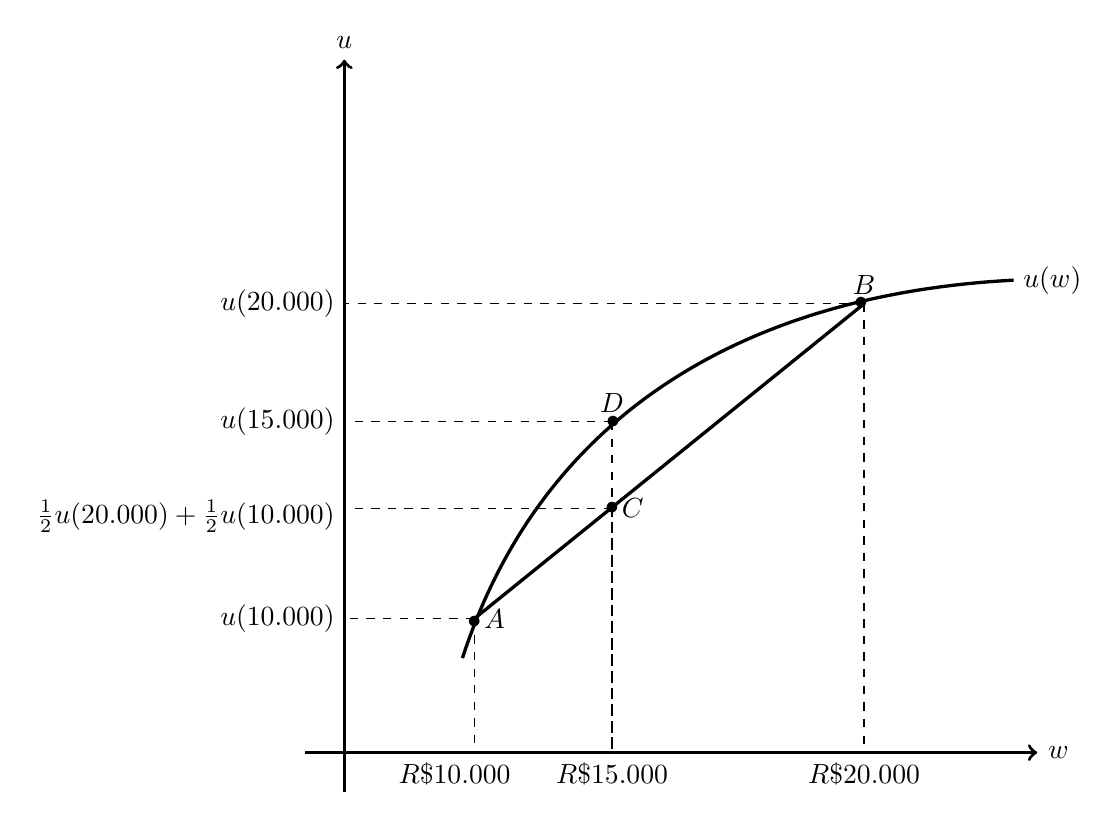
\begin{tikzpicture}[scale=1]  %Inicio Gráfico e tamanho da escala
						%Eixos
					\draw[->, very thick] (-0.5,0) -- (8.8,0) node[right]{$w$}; %Eixo X1
					\draw[->, very thick] (0,-0.5) -- (0,8.8) node[above]{$u$}; %Eixo X2					
					    %Curva
                        \draw[very thick] (1.5,1.2) to [out=72,in=183] (8.5,6);
                        \node[right] at (8.5,6) {$u(w)$};
                         
                        \draw[very thick] (1.65,1.7)--(6.6,5.7);
					
						%Complementos gráficos
		            \draw[dashed] (1.65,1.7) -- (1.65,0); %Pontilhado eixo X1
                    \draw[dashed] (1.65,1.7) -- (0,1.7); %Pontilhado eixo X2
                    \node[left] at (0,1.7) {$u(10.000)$};
                    \node[below] at (1.65,0) {$ R\$ 10.000 \hspace{0.5cm}$};
                    \node[right] at (1.65,1.7) {$A$};
                     \node[above] at (1.65,1.45) {$\bullet$};
                    
                   
                    \draw[dashed] (3.4,3.1) -- (3.4,0); %Pontilhado eixo X1
                    \draw[dashed] (3.4,3.1) -- (0,3.1); %Pontilhado eixo X2
                    \node[left] at (0,3) {$\frac{1}{2}u(20.000)+\frac{1}{2}u(10.000)$};
                    \node[right] at (3.4,3.1) {$C$};
                    \node[above] at (3.4,2.9) {$\bullet$};
                     
                    \draw[dashed] (3.4,4.2) -- (3.4,0); %Pontilhado eixo X1
                    \draw[dashed] (3.4,4.2) -- (0,4.2); %Pontilhado eixo X2
                    \node[left] at (0,4.2) {$u(15.000)$};
                    \node[below] at (3.4,0) {$ R\$ 15.000$};
                    \node[above] at (3.4,4.2) {$D$};
                     \node[right] at (3.2,4.2) {$\bullet$};
                    
                    \draw[dashed] (6.6,5.7) -- (6.6,0); %Pontilhado eixo X1
                    \draw[dashed] (6.6,5.7) -- (0,5.7); %Pontilhado eixo X2
                    \node[left] at (0,5.7) {$u(20.000)$};
                    \node[below] at (6.6,0) {$ R\$ 20.000$};
                    \node[above] at (6.6,5.7) {$B$};
                     \node[right] at (6.35,5.7) {$\bullet$};
                    
                
				\end{tikzpicture} %Fim do gráfico
\end{center}

\paragraph{} b) Suponha agora que existem dois tipos de seguros disponíveis: i) um seguro justo que cobre a perda total, ii) seguro justo que cobre metade da perda total. Calcule o preço do seguro ii) e mostre que indivíduos avessos ao risco preferem o primeiro ao segundo.\\

\textbf{Resposta:}\\

O preço atuarialmente justo do seguro (P2) que cobre só a metade da perda é:
{$P = 0,5 * 5.000 = 2.500$}

A utilidade do indivíduo com este seguro {$(U_{m})$} é:

{$U_{m} = 0,5u(20.000 - 2.500) + 0,5u(20.000 - 2.500 - 10.000 + 5.000) = 0,5u(17.500)+0,5u(12.500)$}\\

Como {$u$} é estritamente côncava, vale que:\\

{$U_{cs} = u(15.000) > 0,5u(17.500) + 0,5u(12.500) = U_m$}\\

O indivíduo prefere o seguro total, em que ele consegue eliminar totalmente o risco e obter a mesma utilidade qualquer que seja o estado da natureza que ocorra. Com o segundo seguro, o indivíduo consegue apenas diminuir um pouco a variação na sua renda, mas nã consegue eliminar totalmente o risco. Logo, sua utilidade será maior com o seguro total do que com o seguro parcial.\\

\item[10.] (A09) Um indivíduo possui uma função de utilidade de Bernoulli dada por {$u(w) = 1 - (1/w)$}, em que {$w$} denota o valor presente líquido da sua renda futura. No momento, ele está contemplando duas opções de carreira prossional. A primeira opção dará a ele uma renda certa de {$w = 5$}. A outra alternativa dará {$w = 400$}, com 1\% de chance, e {$w = 4$} com 99\% de chance. Responda aos seguintes itens:\\


\paragraph{} b) Calcule a utilidade esperada das duas opções. Qual deve ser a escolha desse indivíduo?\\

\textbf{Resposta:}\\

Utilidade esperada da 1ª opção: {$ U(1) = 1 - 1/5 = 4/5 = 0,8.$}\\

Utilidade esperada da 2ª opção: {$ U(2) = \dfrac{1}{100} \left( 1 - \dfrac{1}{400} \right) + \dfrac{99}{100} \left( 1 - \dfrac{1}{4} \right) = \dfrac{1}{100} \left(\dfrac{399}{400} \right) + \dfrac{99}{100} \left(\dfrac{3}{4} \right) = \dfrac{1}{400} (3,99 + 297) = \dfrac{300,99}{400} \approx \dfrac{3}{4}$}\\

Como {$4/5 > 3/4$} a utilidade da primeira opção é maior.



\end{enumerate}

